\documentclass[14pt,c]{beamer}
\setbeamertemplate{caption}[numbered]
\setbeamertemplate{caption label separator}{: }
\setbeamercolor{caption name}{fg=normal text.fg}
\beamertemplatenavigationsymbolsempty
\usepackage{lmodern}
\usepackage{amssymb,amsmath}
\usepackage{framed}
\usepackage{parskip}
\definecolor{shadecolor}{RGB}{200,200,200}
\usepackage{multicol}
\usepackage{multirow}
\usepackage{tabularx}
\usepackage[norsk]{babel}
\usepackage[utf8]{inputenc}
\newcolumntype{C}{>{\centering\arraybackslash}X}
% Theme
\mode<presentation>
{
  \usetheme{Honefoss}
}

\defbeamertemplate*{title page}{kartverket2 theme}[1][]{
\vspace*{15pt}
\hspace*{-5mm}
    \begin{minipage}{\textwidth}
      \begin{beamercolorbox}[sep=10pt,left,#1]{title}
        \usebeamerfont{title}\inserttitle\par%
        \ifx\insertsubtitle\@empty%
        \else%
        \vskip0.4em%
               {\usebeamerfont{subtitle}\usebeamercolor[fg]{subtitle}\insertsubtitle\par}%
               \fi%     
      \end{beamercolorbox}%
      \vspace*{2mm}
      \begin{beamercolorbox}[sep=10pt,left,#1]{author}
        \usebeamerfont{author}\insertauthor
      \end{beamercolorbox}
      \vfill%
    \end{minipage}
}

\raggedbottom

\setlength{\parindent}{0pt}
\setlength{\parskip}{6pt plus 2pt minus 1pt}
\providecommand{\tightlist}{%
  \setlength{\itemsep}{0pt}\setlength{\parskip}{0pt}}
\setcounter{secnumdepth}{0}

\setbeamercolor{title}{fg=white}
\title{VLBI analyse i Kartverket}
\setbeamercolor{author}{fg=kvlightblue}
\author{Ann-Silje~Kirkvik \\ Geir~Arne~Hjelle \\ Michael~D\"ahnn \\ Ingrid~Fausk}

\begin{document}
{
    \usebackgroundtemplate{
        %
        \centering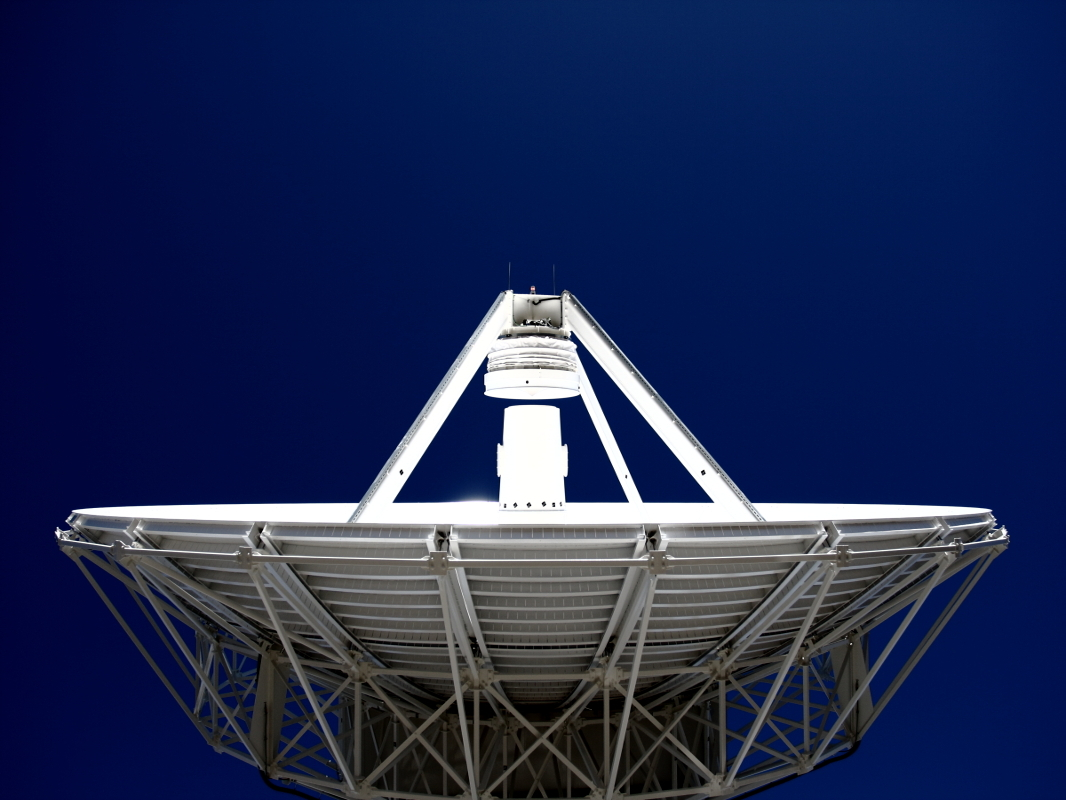
\includegraphics[height=\paperheight]{figure/nyal9}
    }
    \frame[plain,t]{\titlepage}
}

\begin{frame}{Kort historie}
  \begin{itemize}
    \item VLBI analyse startet med GEOSAT ifra FFI
    \item Ble et assosiert IVS analysesenter i 2010
    \item Prøvde å bidra til ITRF2014 med GEOSAT
    \item Prøvde å bidra til VASCC2015 med GEOSAT
    \item GEOSAT ble til slutt lagt på hylla i 2015
    \item \textbf{Where} ble startet på i 2015
  \end{itemize}
\end{frame}


\begin{frame}{ITRF2014}
\begin{itemize}
  \item Analyserte 24 timers sesjoner fra 1994-2014
  \item Flere iterasjoner med leveranser til IVS
  \begin{itemize}
    \item Feil i bruk av kabelkalibreringsdata
    \item Feil i bruk av eksentrisitetsvektorer
	\item Feil i håndtering av søsken-antenner
	\item Altfor sterke føringer i estimeringen 
	\end{itemize}
  \item Gikk tom for tid til feilretting
  \item Den siste løsningen måtte trekkes tilbake
\end{itemize}
\end{frame}


\begin{frame}{VASCC 2015}
 The VLBI Analysis Software Comparison Campaign
\begin{small}
  \begin{itemize}
    \item Utført av Grzegorz Klopotek ved Chalmers
    \item Sammenligner VLBI modellen i forskjellige programvarer
    \item VLBI modellen er en viktig del av en VLBI analyse, men den er ikke alt
    \item VLBI modellen består av flere deler (som ble testet hver for seg)
  \end{itemize}
\end{small}
\end{frame}


\begin{frame}{VASCC resultater}
 \begin{small}
  \begin{itemize}
    \item 11 deltakere i kampanjen
    \item 6 av 11 løsninger var konsistente innenfor 1~mm
    \item Kartverket deltok med løsninger ifra GEOSAT
    \item Etter mye graving og feilretting ble enkelte deler av VLBI modellen i GEOSAT konsistent
    \item Klarte ikke å få konsistente løsninger for hele VLBI modellen med GEOSAT
    \item Fikk tak i 2 av de 6 konsistente løsningene
    \item Sammenlignet Where med disse to løsningene i 2017
  \end{itemize}
 \end{small}
\end{frame}


\begin{frame}{\textbf{Where} vs VieVS and c5++}
  \begin{itemize}
    \item 2 nettverk, 2 radiokilder 
    \item 16 dager, 1 min observasjoner
  \end{itemize}
\vspace{5pt}
RMS (i mm) av forskjellen mellom løsningene:
\vspace{1em}

  \begin{tabularx}{\columnwidth}{lrCCC}
  & & \multicolumn{3}{c}{Nord}   \\ \cline{3-5}
  &         & \textbf{Where}  & \textbf{c5++}   & \textbf{VieVS}  \\
  \multirow{3}{*}{\rotatebox[origin=c]{90}{Sør}}
    & \multicolumn{1}{|l}{\textbf{Where}} & $\diamond$ &     $0.49$ &     $0.44$ \\
    & \multicolumn{1}{|l}{\textbf{c5++}}  &     $0.18$ & $\diamond$ &     $0.21$ \\
    & \multicolumn{1}{|l}{\textbf{VieVS}} &     $0.43$ &     $0.39$ & $\diamond$ \\
  \end{tabularx}
\end{frame}


\begin{frame}{IVS analyse senter}
Kartverket har som mål å bli et operasjonelt IVS analysesenter

\begin{itemize}
  \item Jevnlig analysere 24 timers sesjoner innen en tidsfrist
  \item Beregne stasjons- og radiokildekoordinater og jordrotasjonsparametere
  \item Den operasjonelle analysen skal utføres på kontrollsenteret på Hønefoss
  \item Levert 7 testløsninger til kombinasjonssenteret
\end{itemize}
\end{frame}
 
\begin{frame}{Status}
\begin{itemize}
  \item Stasjonskoordinater var godkjent i den 4. leveransen
  \item Radiokildekoordinater var tilsynelatende godkjent i den 5. leveransen, men er ikke tatt inn i kombinasjonen
  enda
  \item Jordrotasjonsparameterne var godkjent i den 6. leveransen
  \item Den 7. leveransen er for å teste overgang til nytt observasjonsfilformat
\end{itemize}
\end{frame}

\begin{frame}{3. leveranse - Ny-{\AA}lesund høyde}
\begin{centering}
    \hfill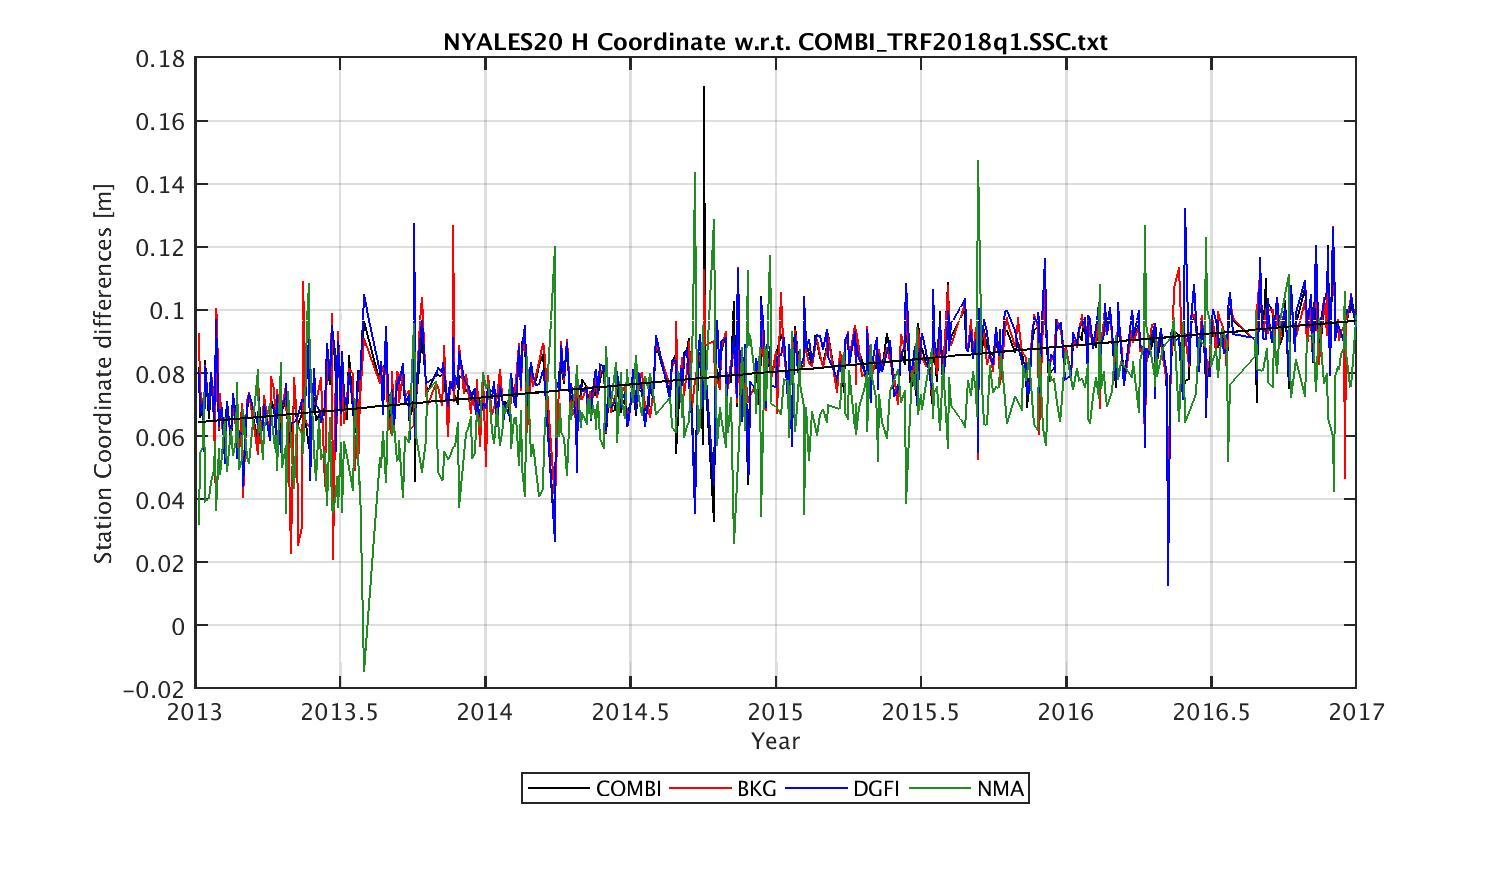
\includegraphics[width=\linewidth]{figure/iter3_NYALES20-H_diff-trf}\hspace*{\fill}
\end{centering}
\end{frame}

\begin{frame}{4. leveranse - Ny-{\AA}lesund høyde}
\begin{centering}
    \hfill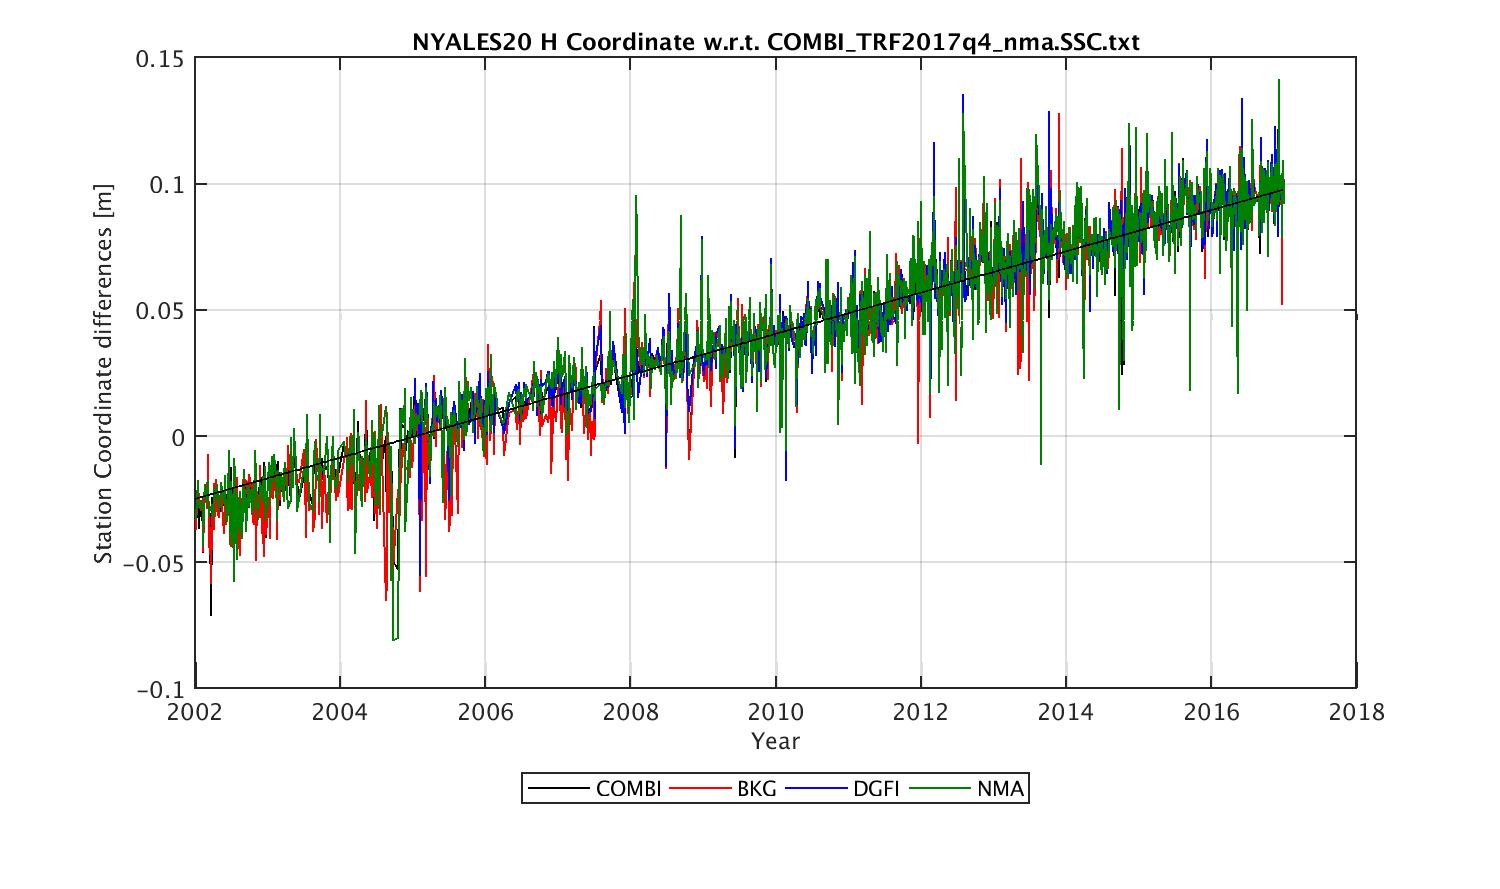
\includegraphics[width=\linewidth]{figure/iter4_NYALES20-H_diff-trf}\hspace*{\fill}
\end{centering}
\end{frame}

\begin{frame}{5. leveranse - LOD}
\begin{centering}
    \hfill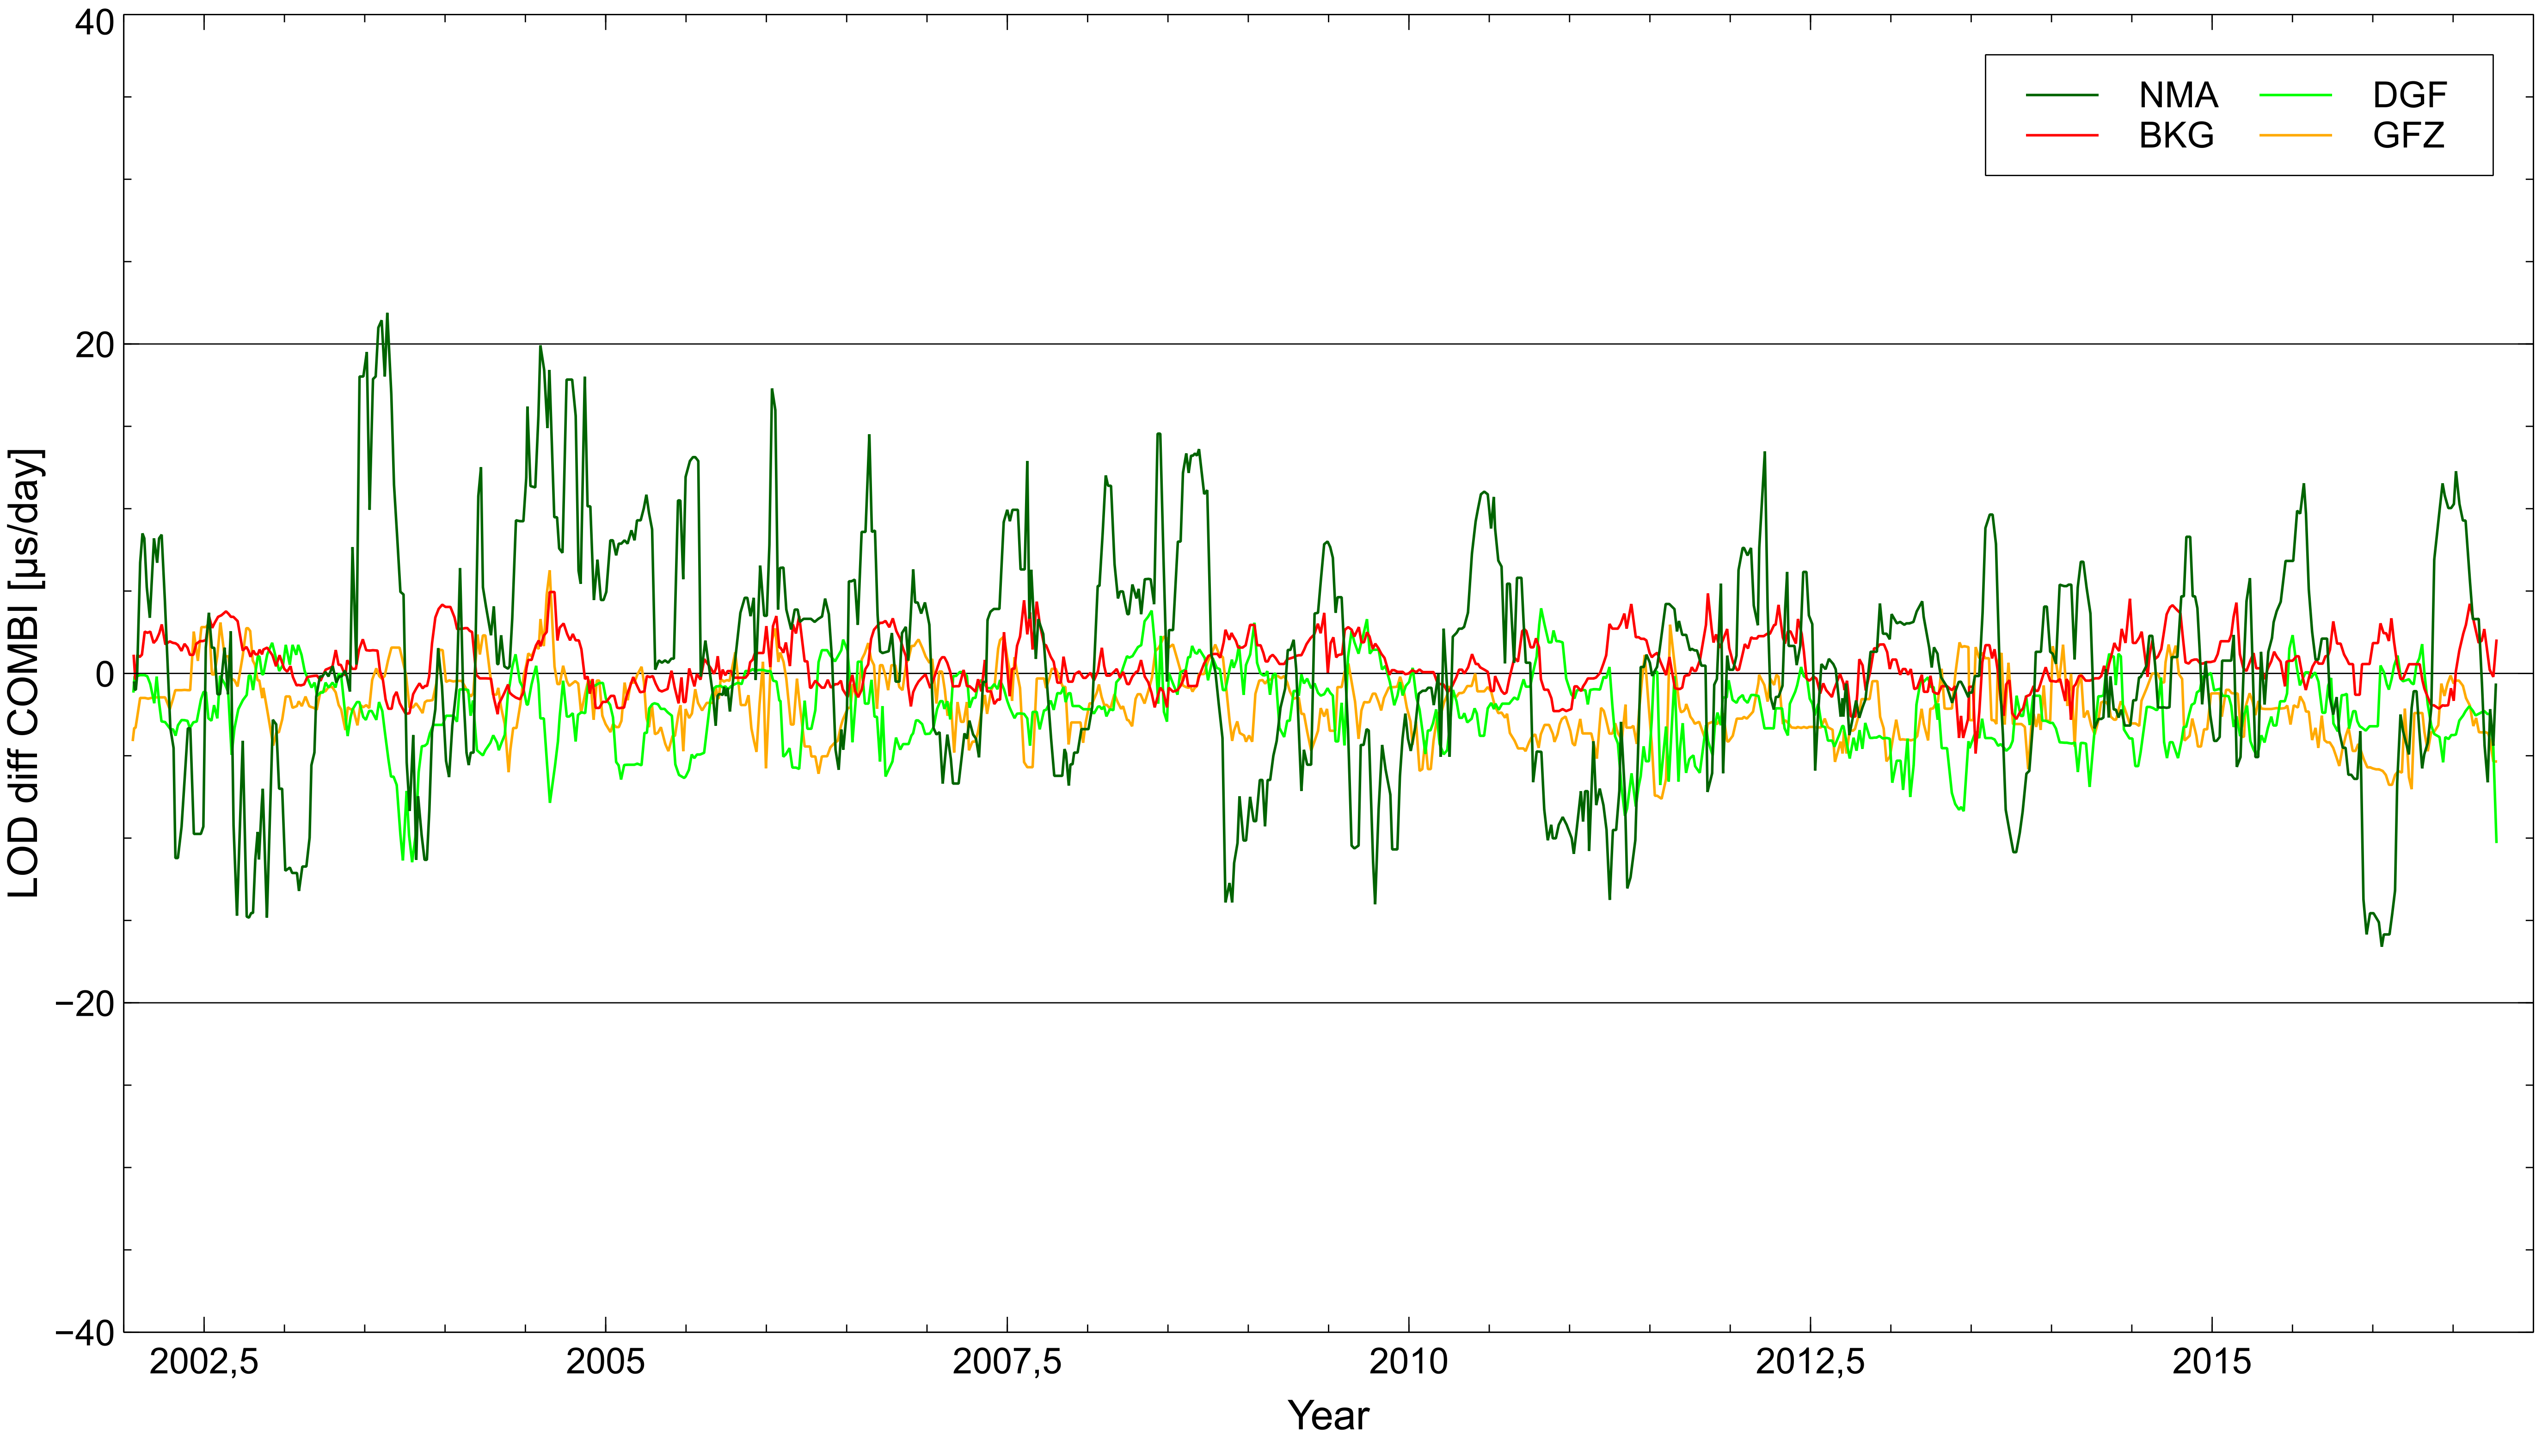
\includegraphics[width=\linewidth]{figure/iter5_lod_nma_diff_combi}\hspace*{\fill}
\end{centering}
\end{frame}

\begin{frame}{6. leveranse - LOD}
\begin{centering}
    \hfill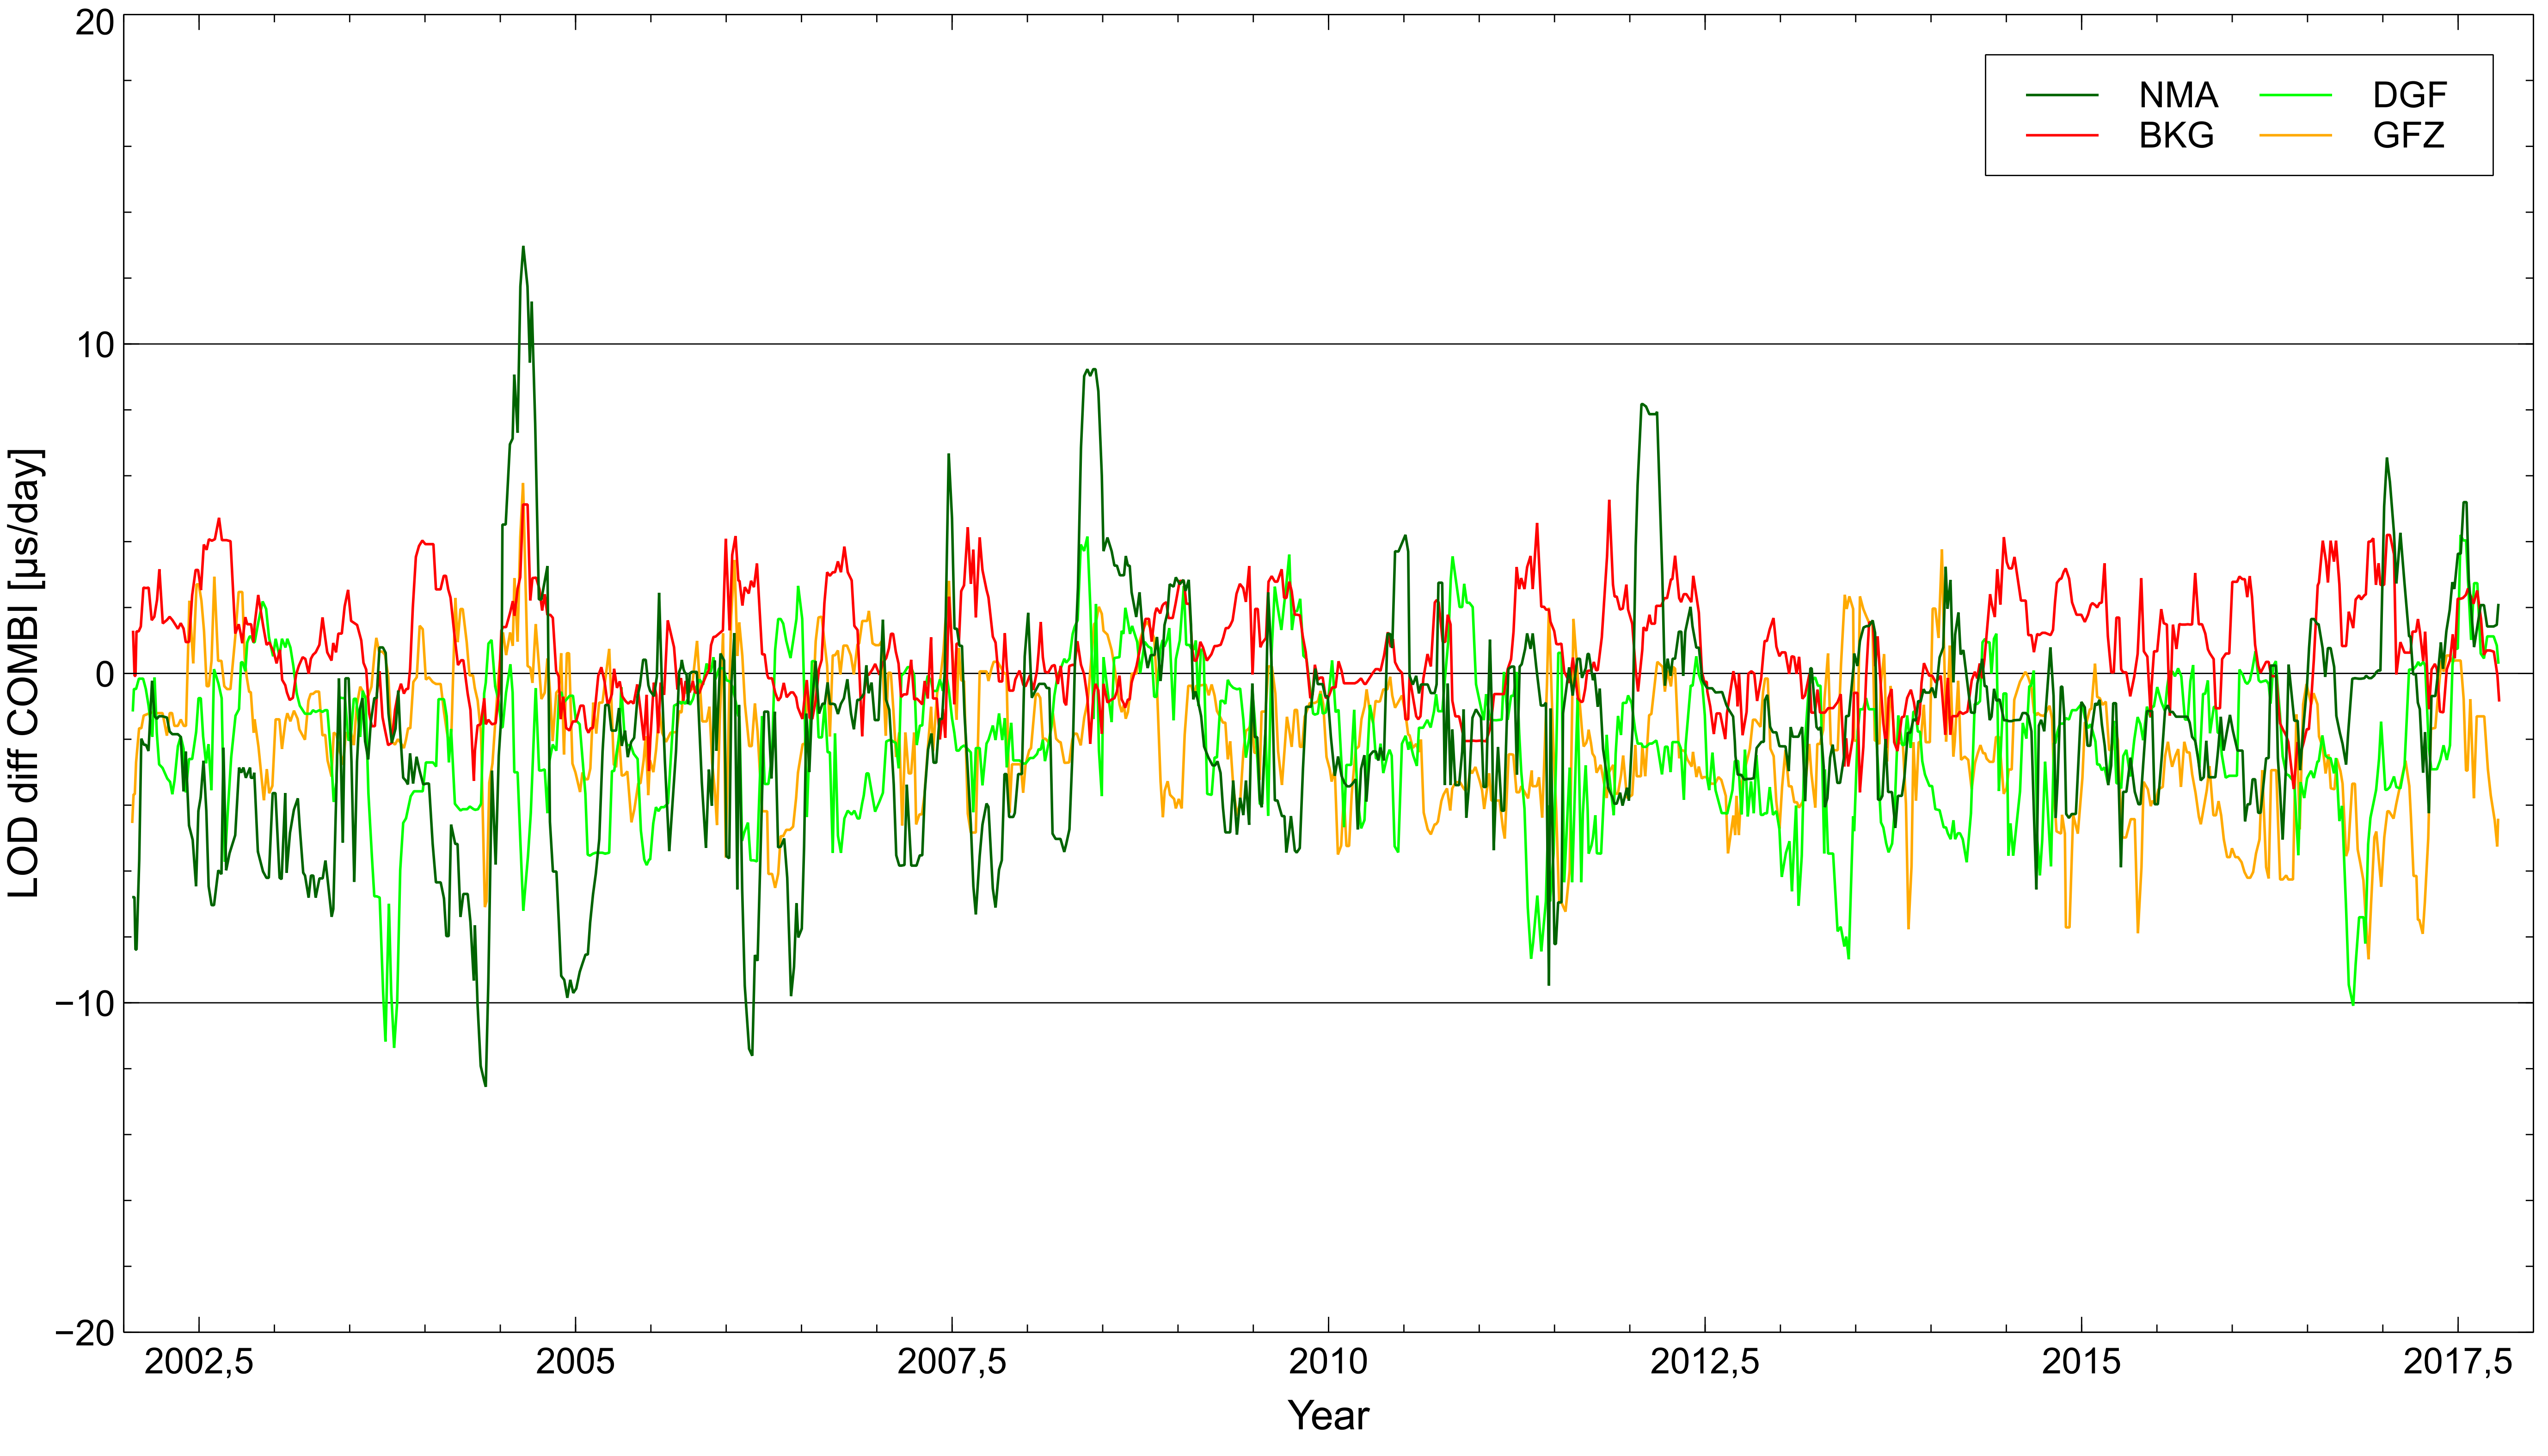
\includegraphics[width=\linewidth]{figure/iter6_lod_nma_diff_combi}\hspace*{\fill}
\end{centering}
\end{frame}

\begin{frame}{5. leveranse - dX}
\begin{centering}
    \hfill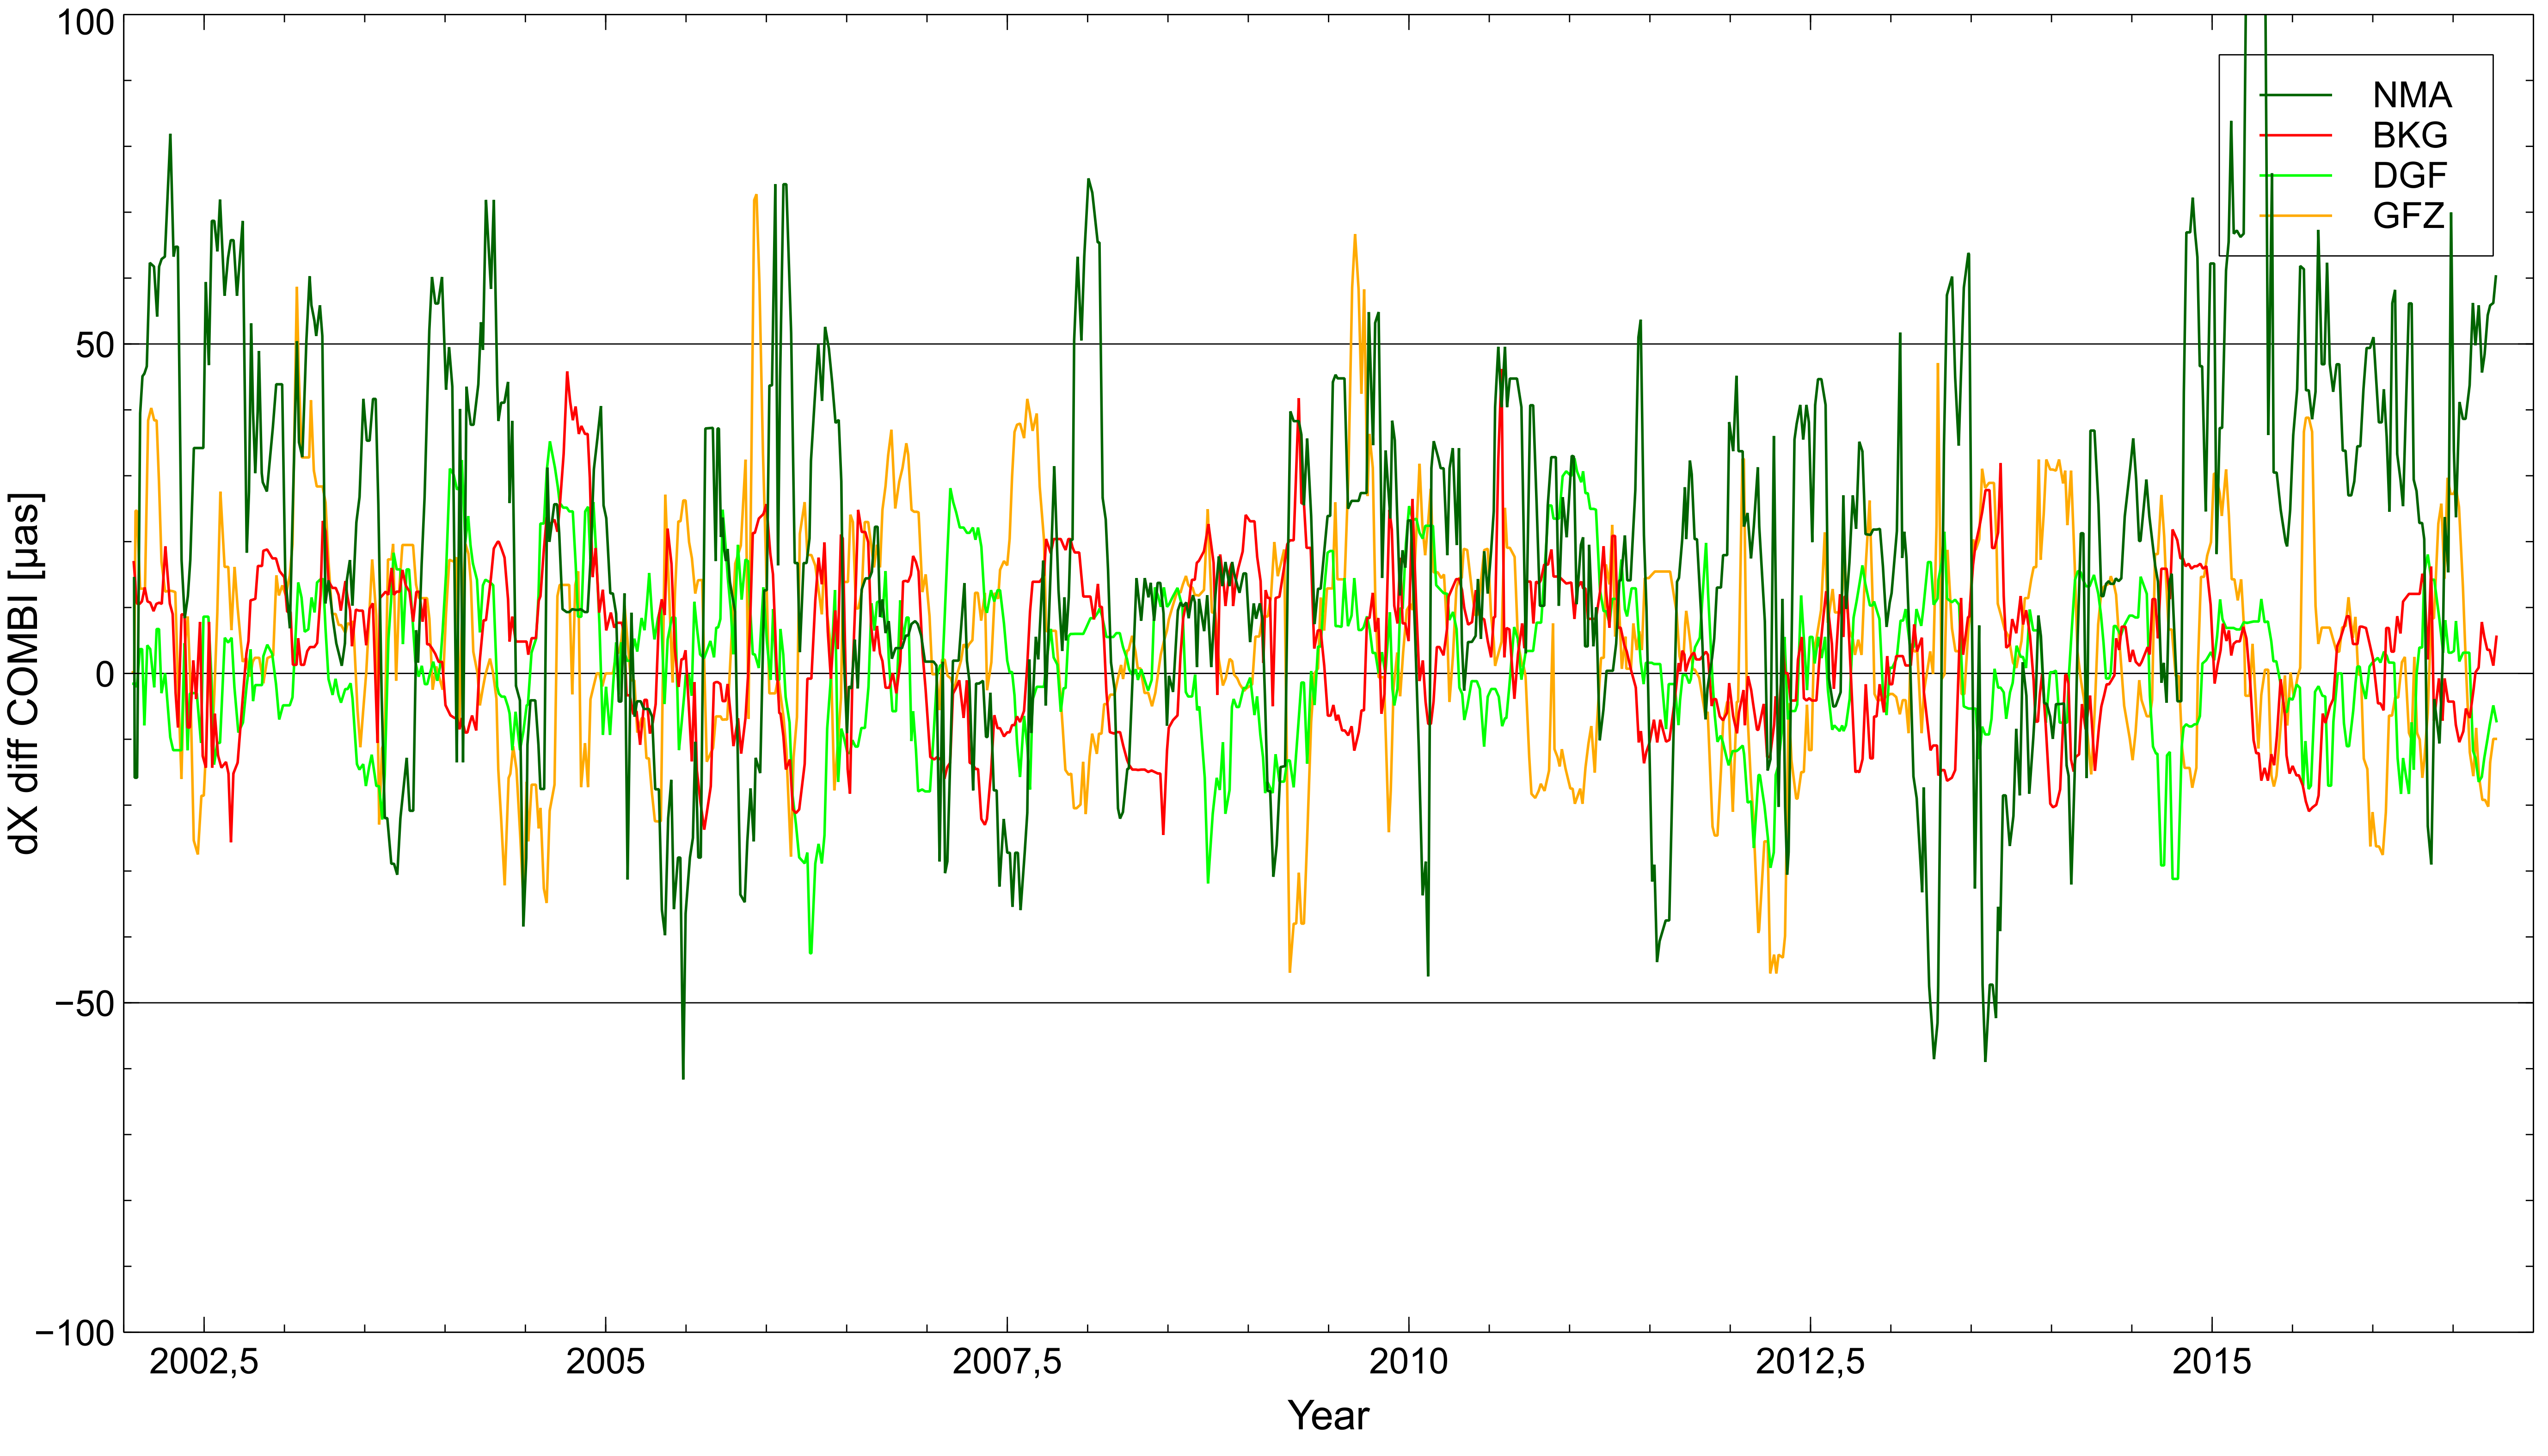
\includegraphics[width=\linewidth]{figure/iter5_dX_nma_diff_combi}\hspace*{\fill}
\end{centering}
\end{frame}

\begin{frame}{6. leveranse - dX}
\begin{centering}
    \hfill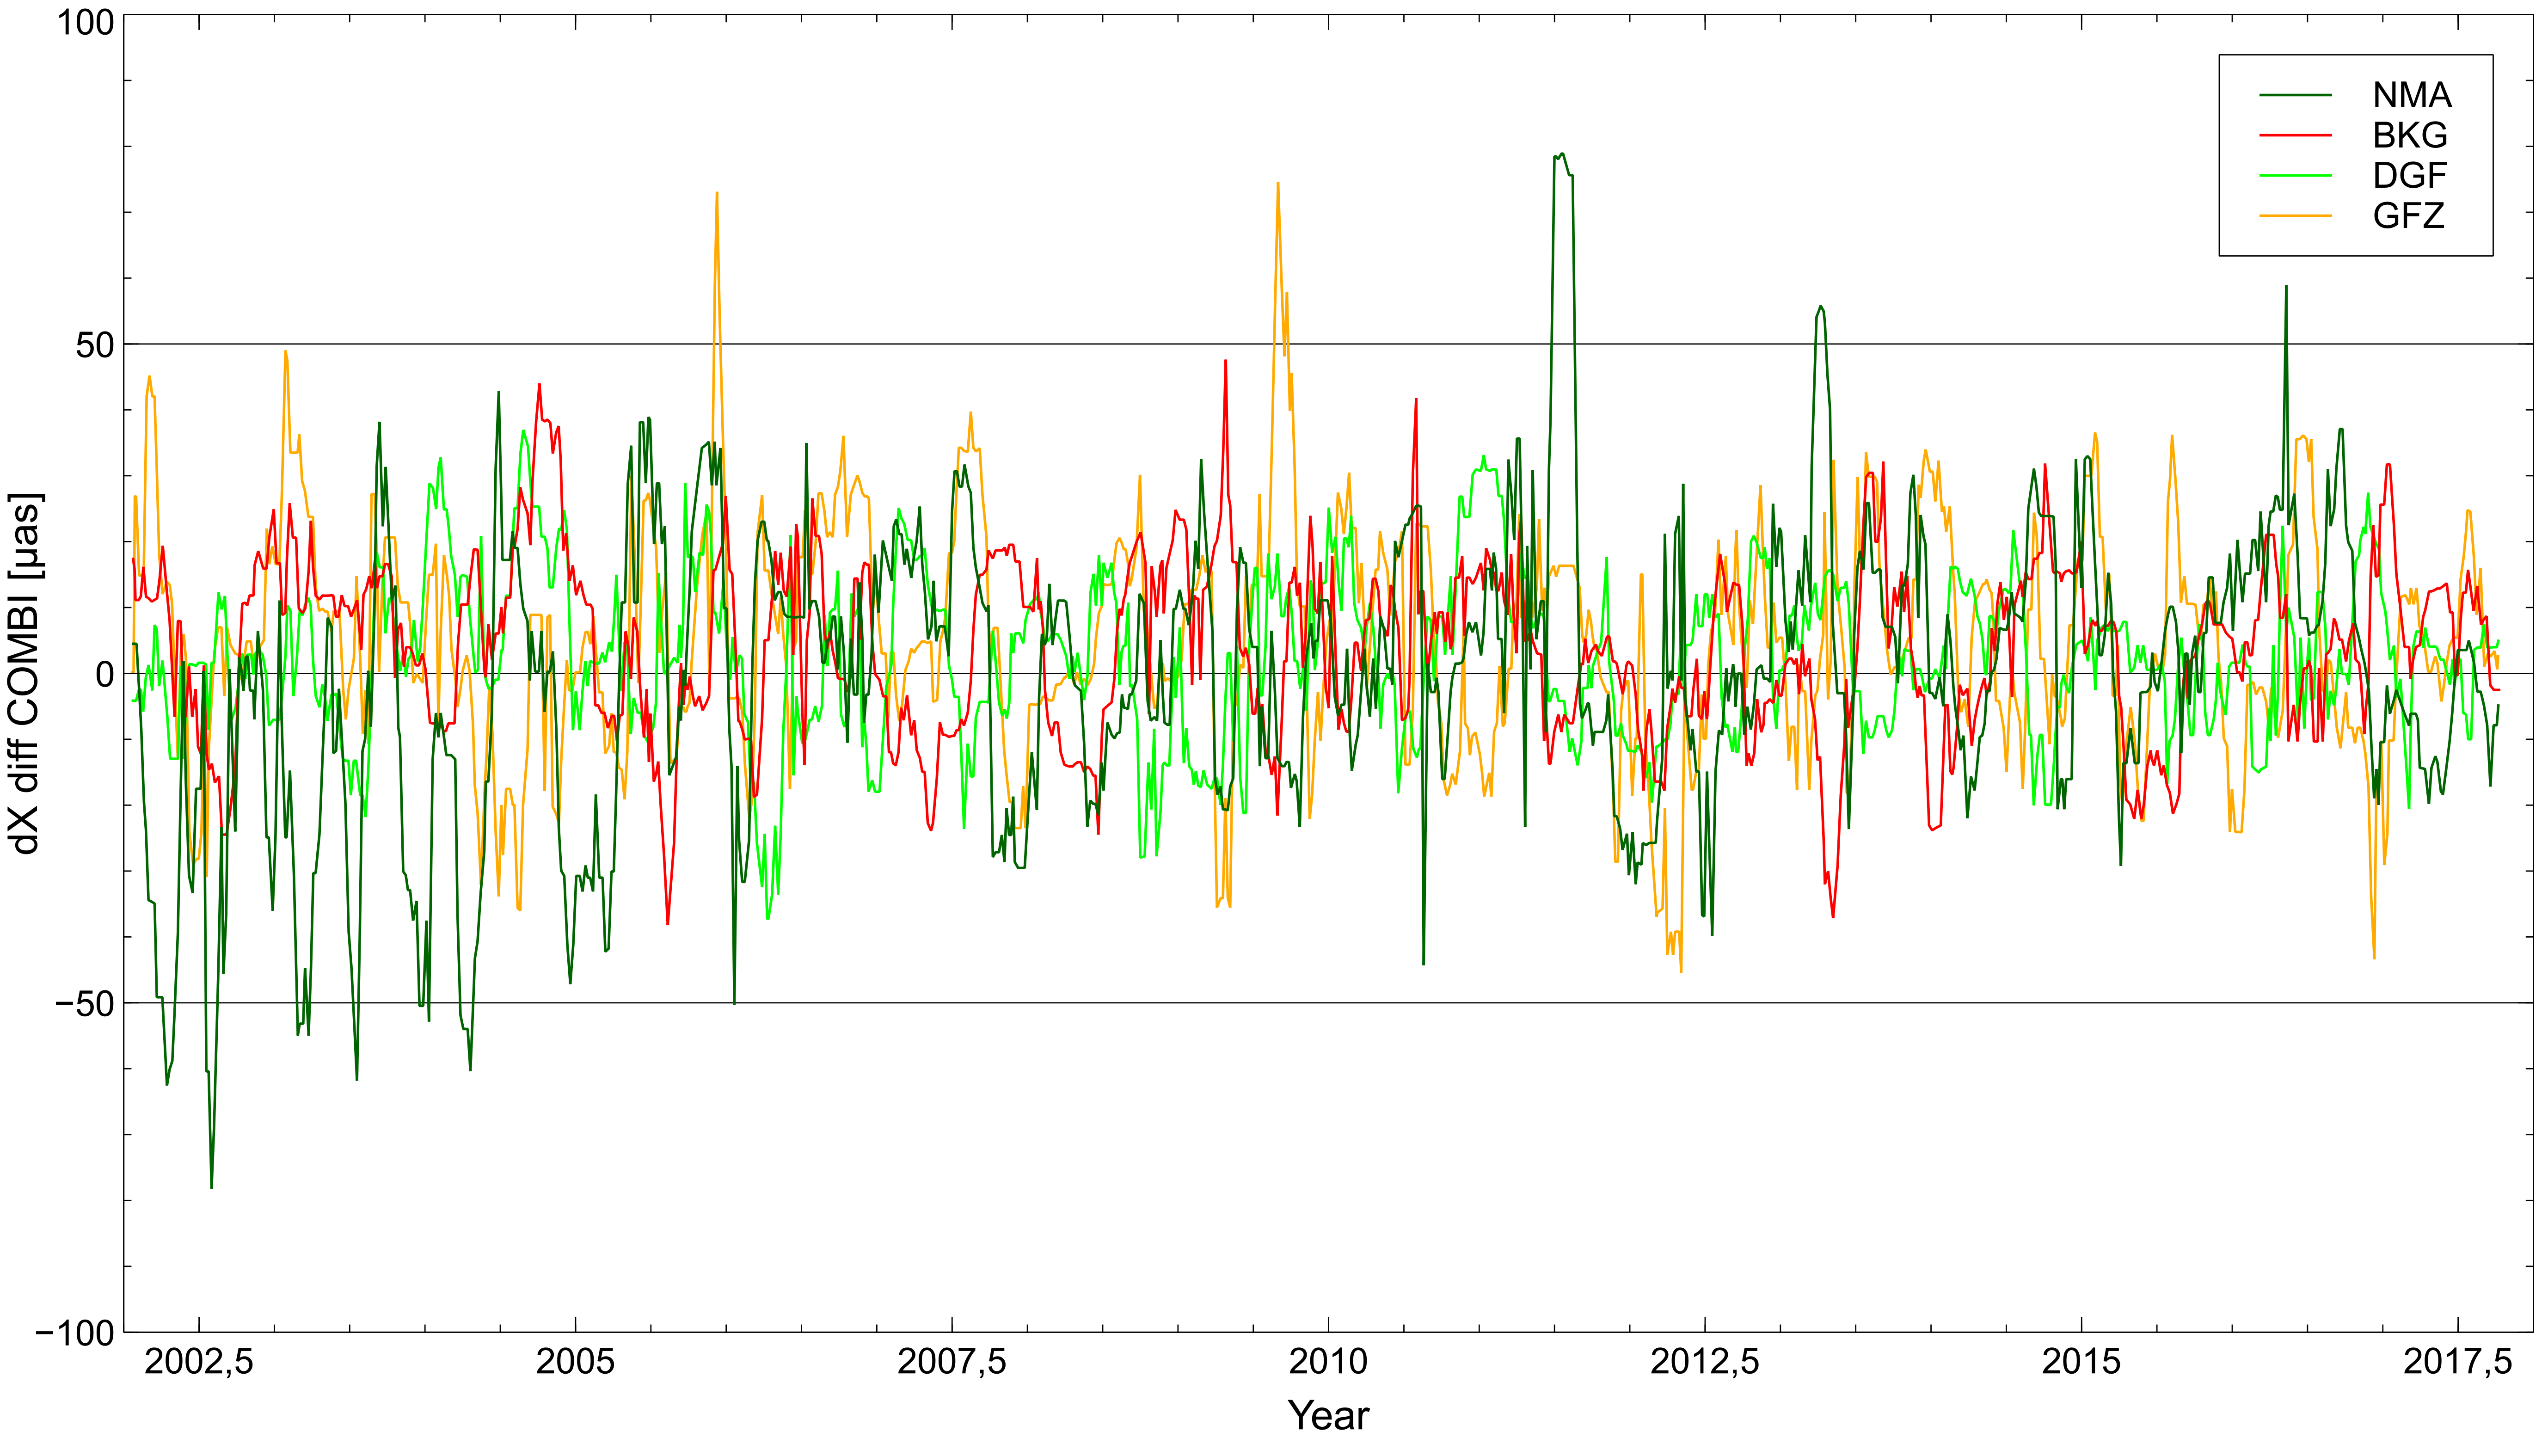
\includegraphics[width=\linewidth]{figure/iter6_dX_nma_diff_combi}\hspace*{\fill}
\end{centering}
\end{frame}

\begin{frame}{6. leveranse - dY}
\begin{centering}
    \hfill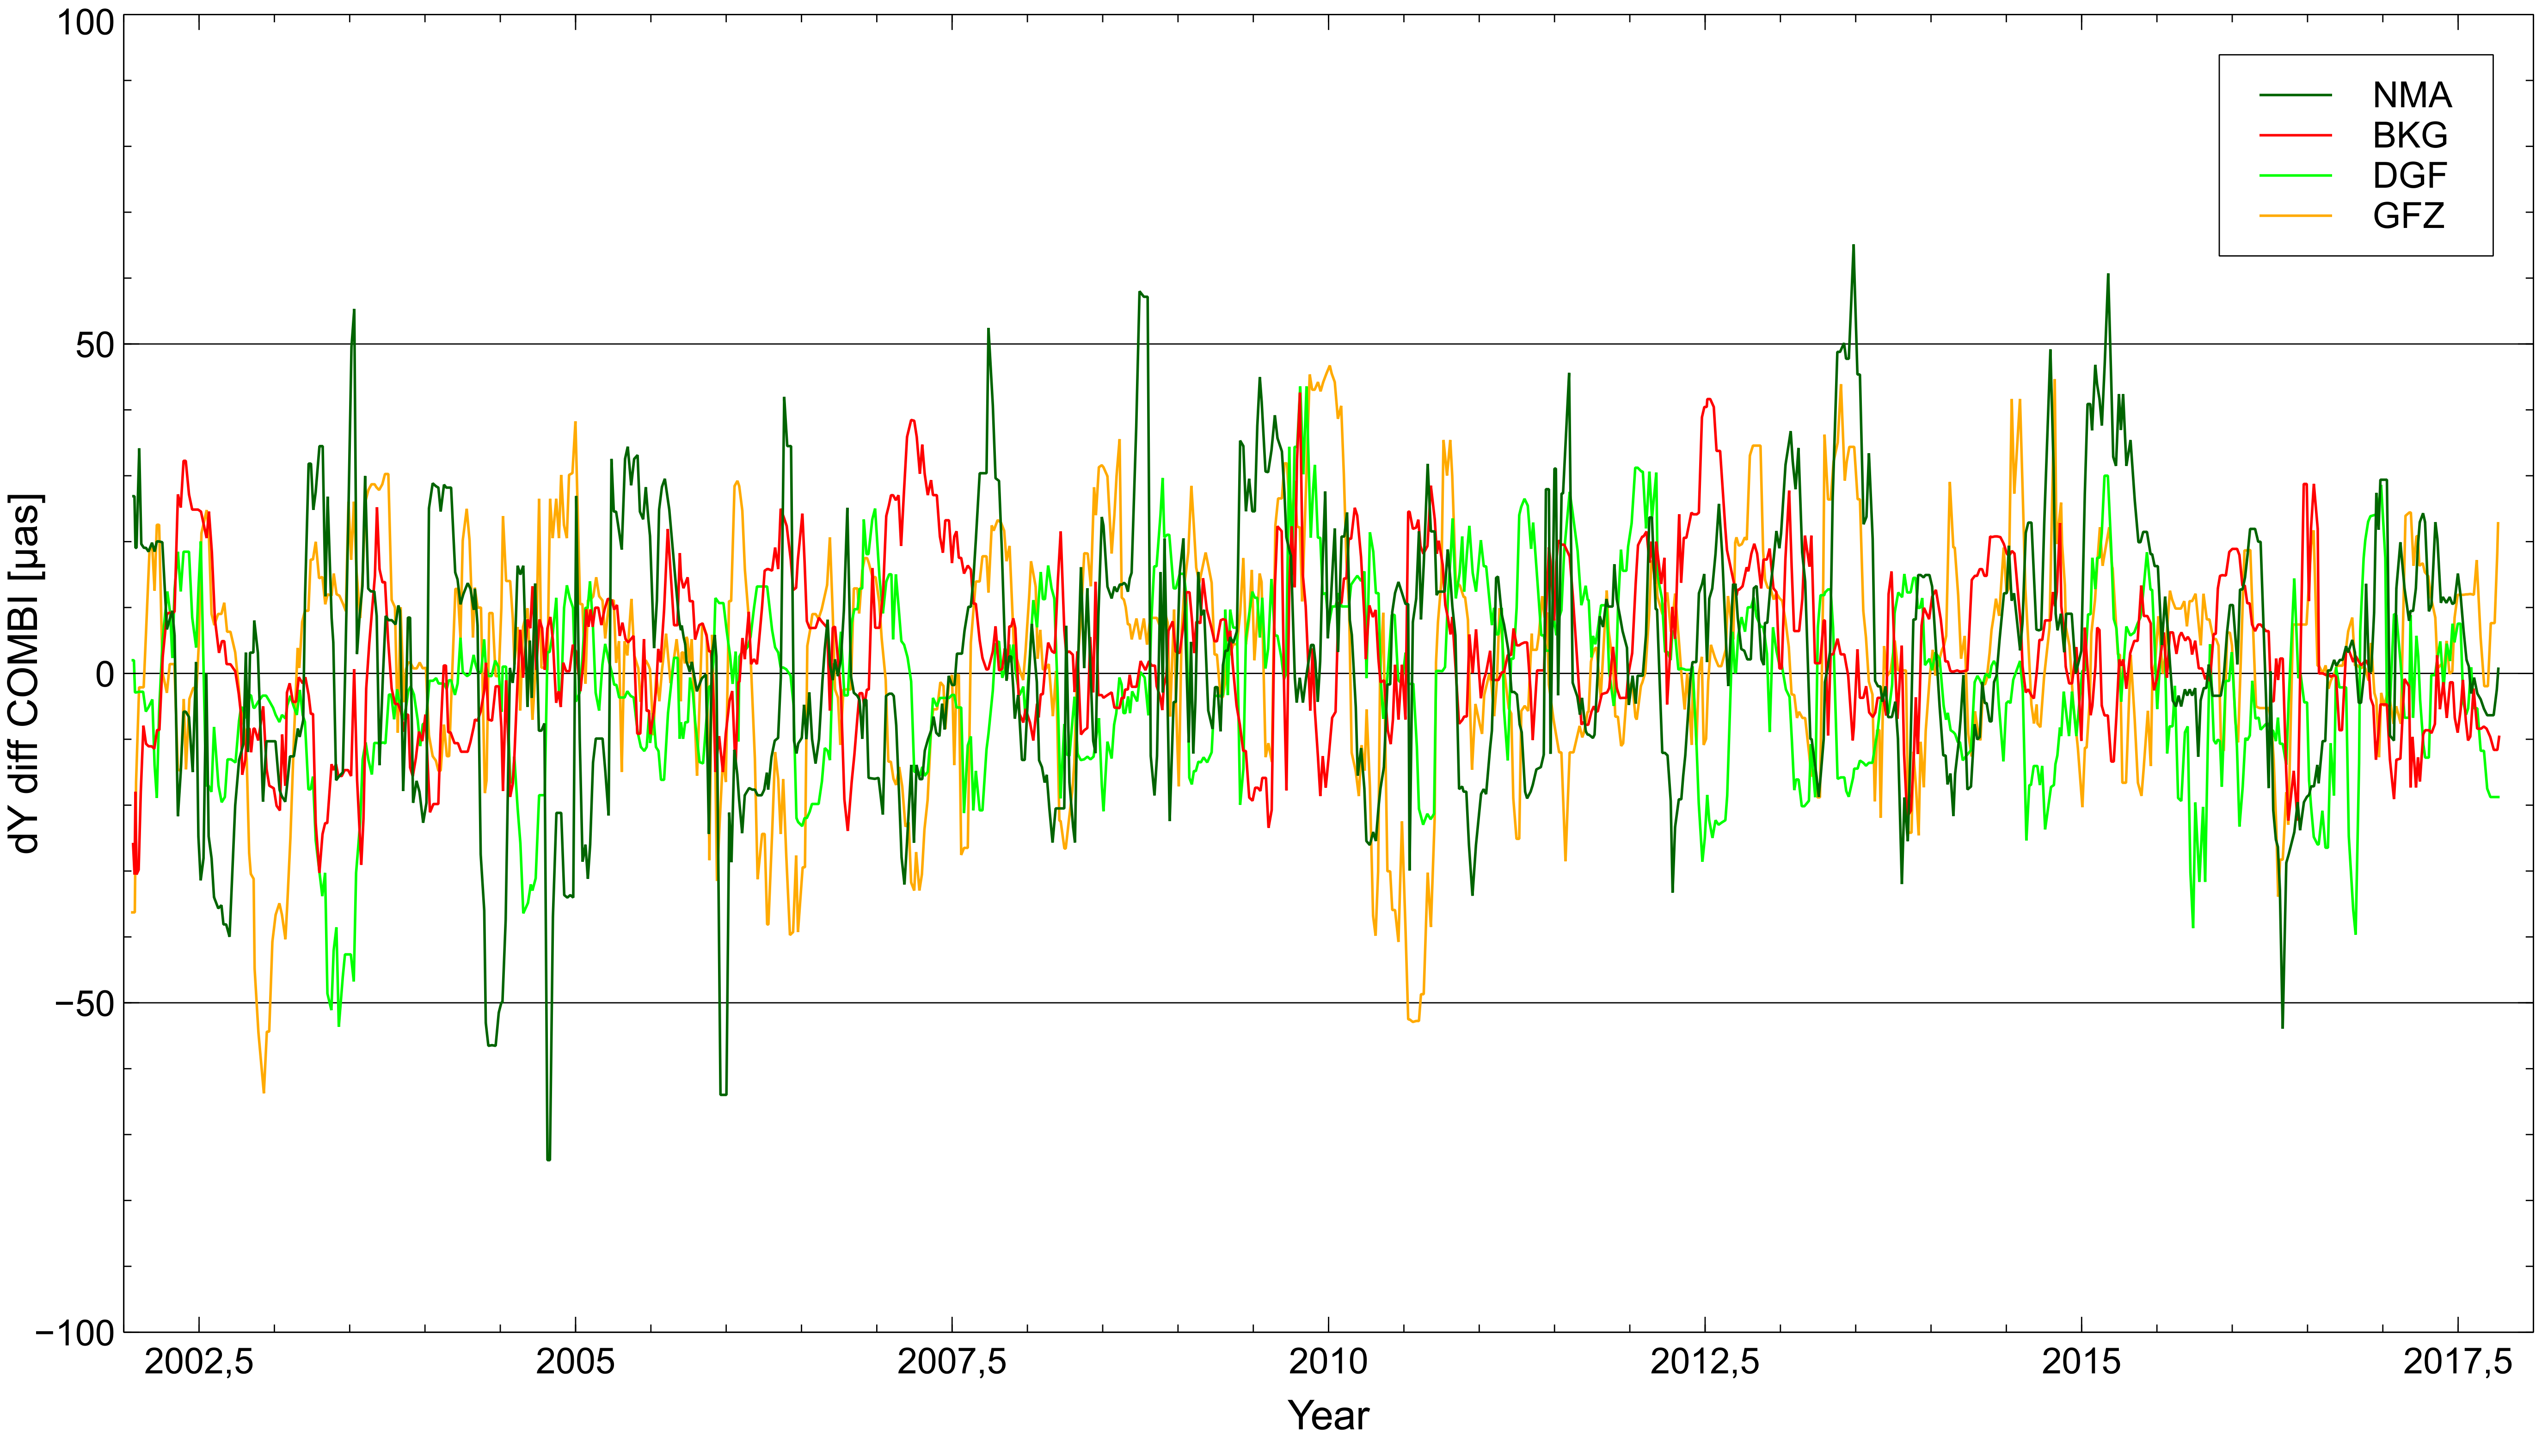
\includegraphics[width=\linewidth]{figure/iter6_dY_nma_diff_combi}\hspace*{\fill}
\end{centering}
\end{frame}

\begin{frame}{6. leveranse - dUT1}
\begin{centering}
    \hfill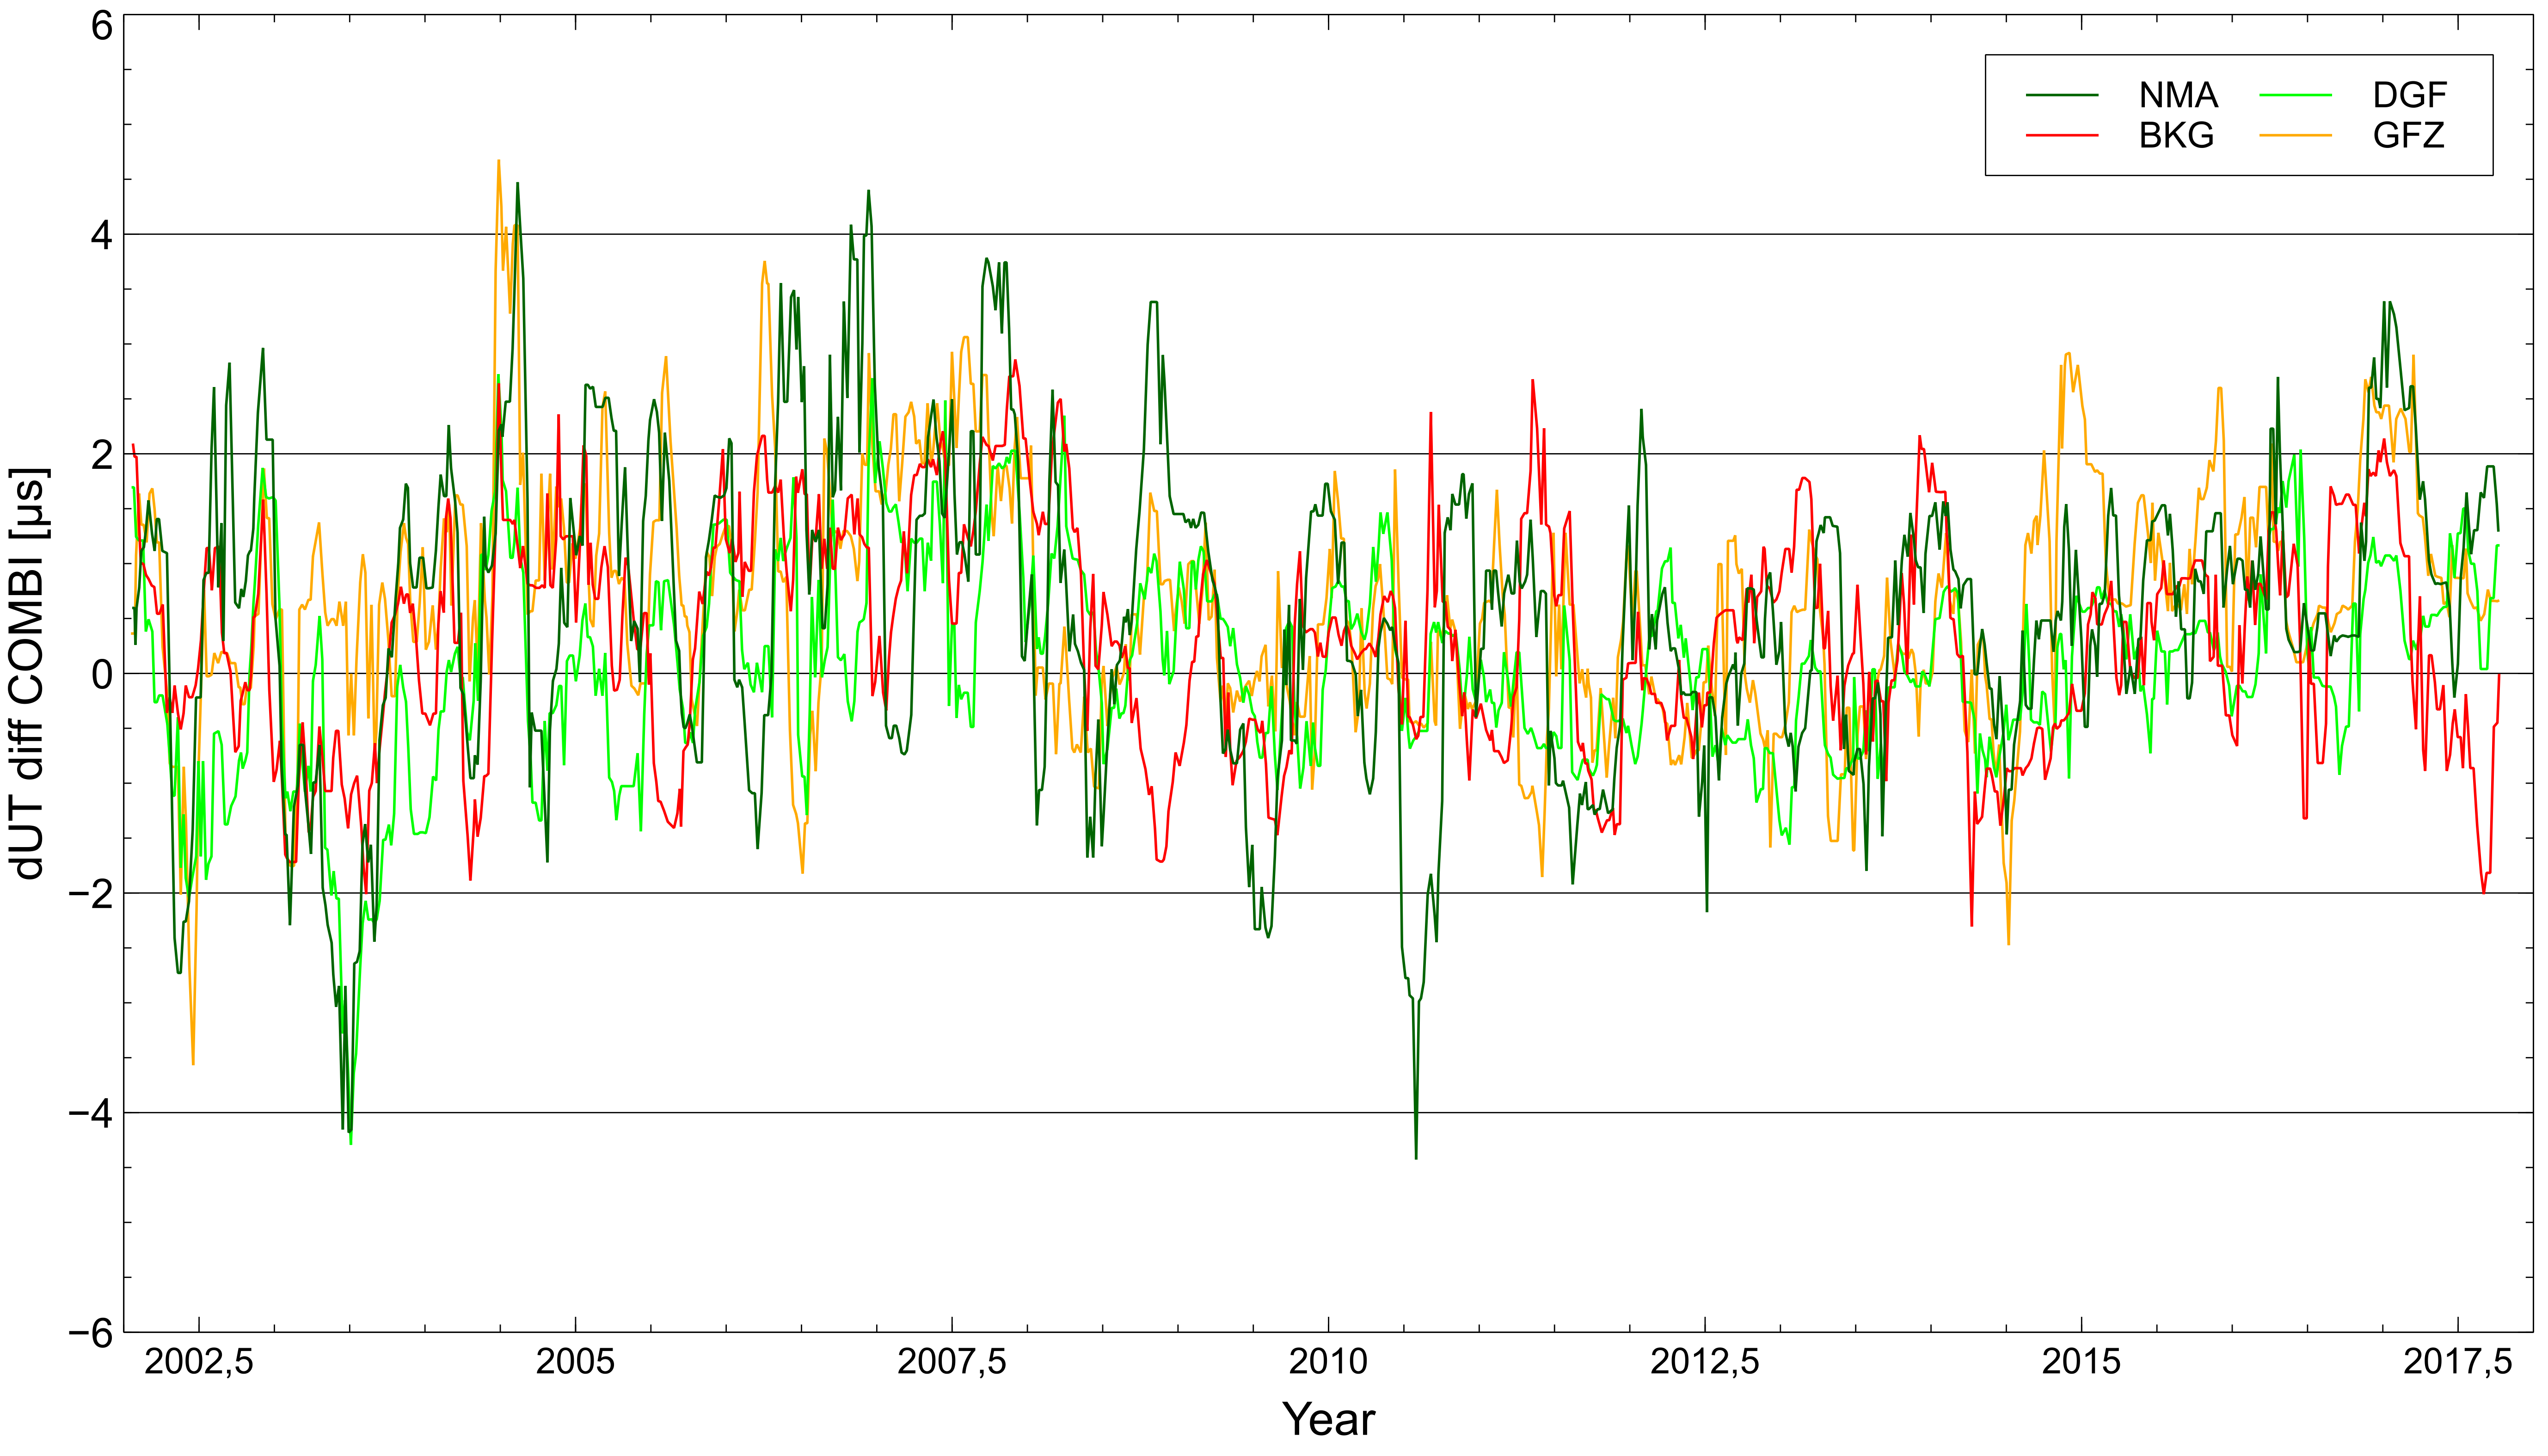
\includegraphics[width=\linewidth]{figure/iter6_dUT_nma_diff_combi}\hspace*{\fill}
\end{centering}
\end{frame}

\begin{frame}{6. leveranse - x-pole}
\begin{centering}
    \hfill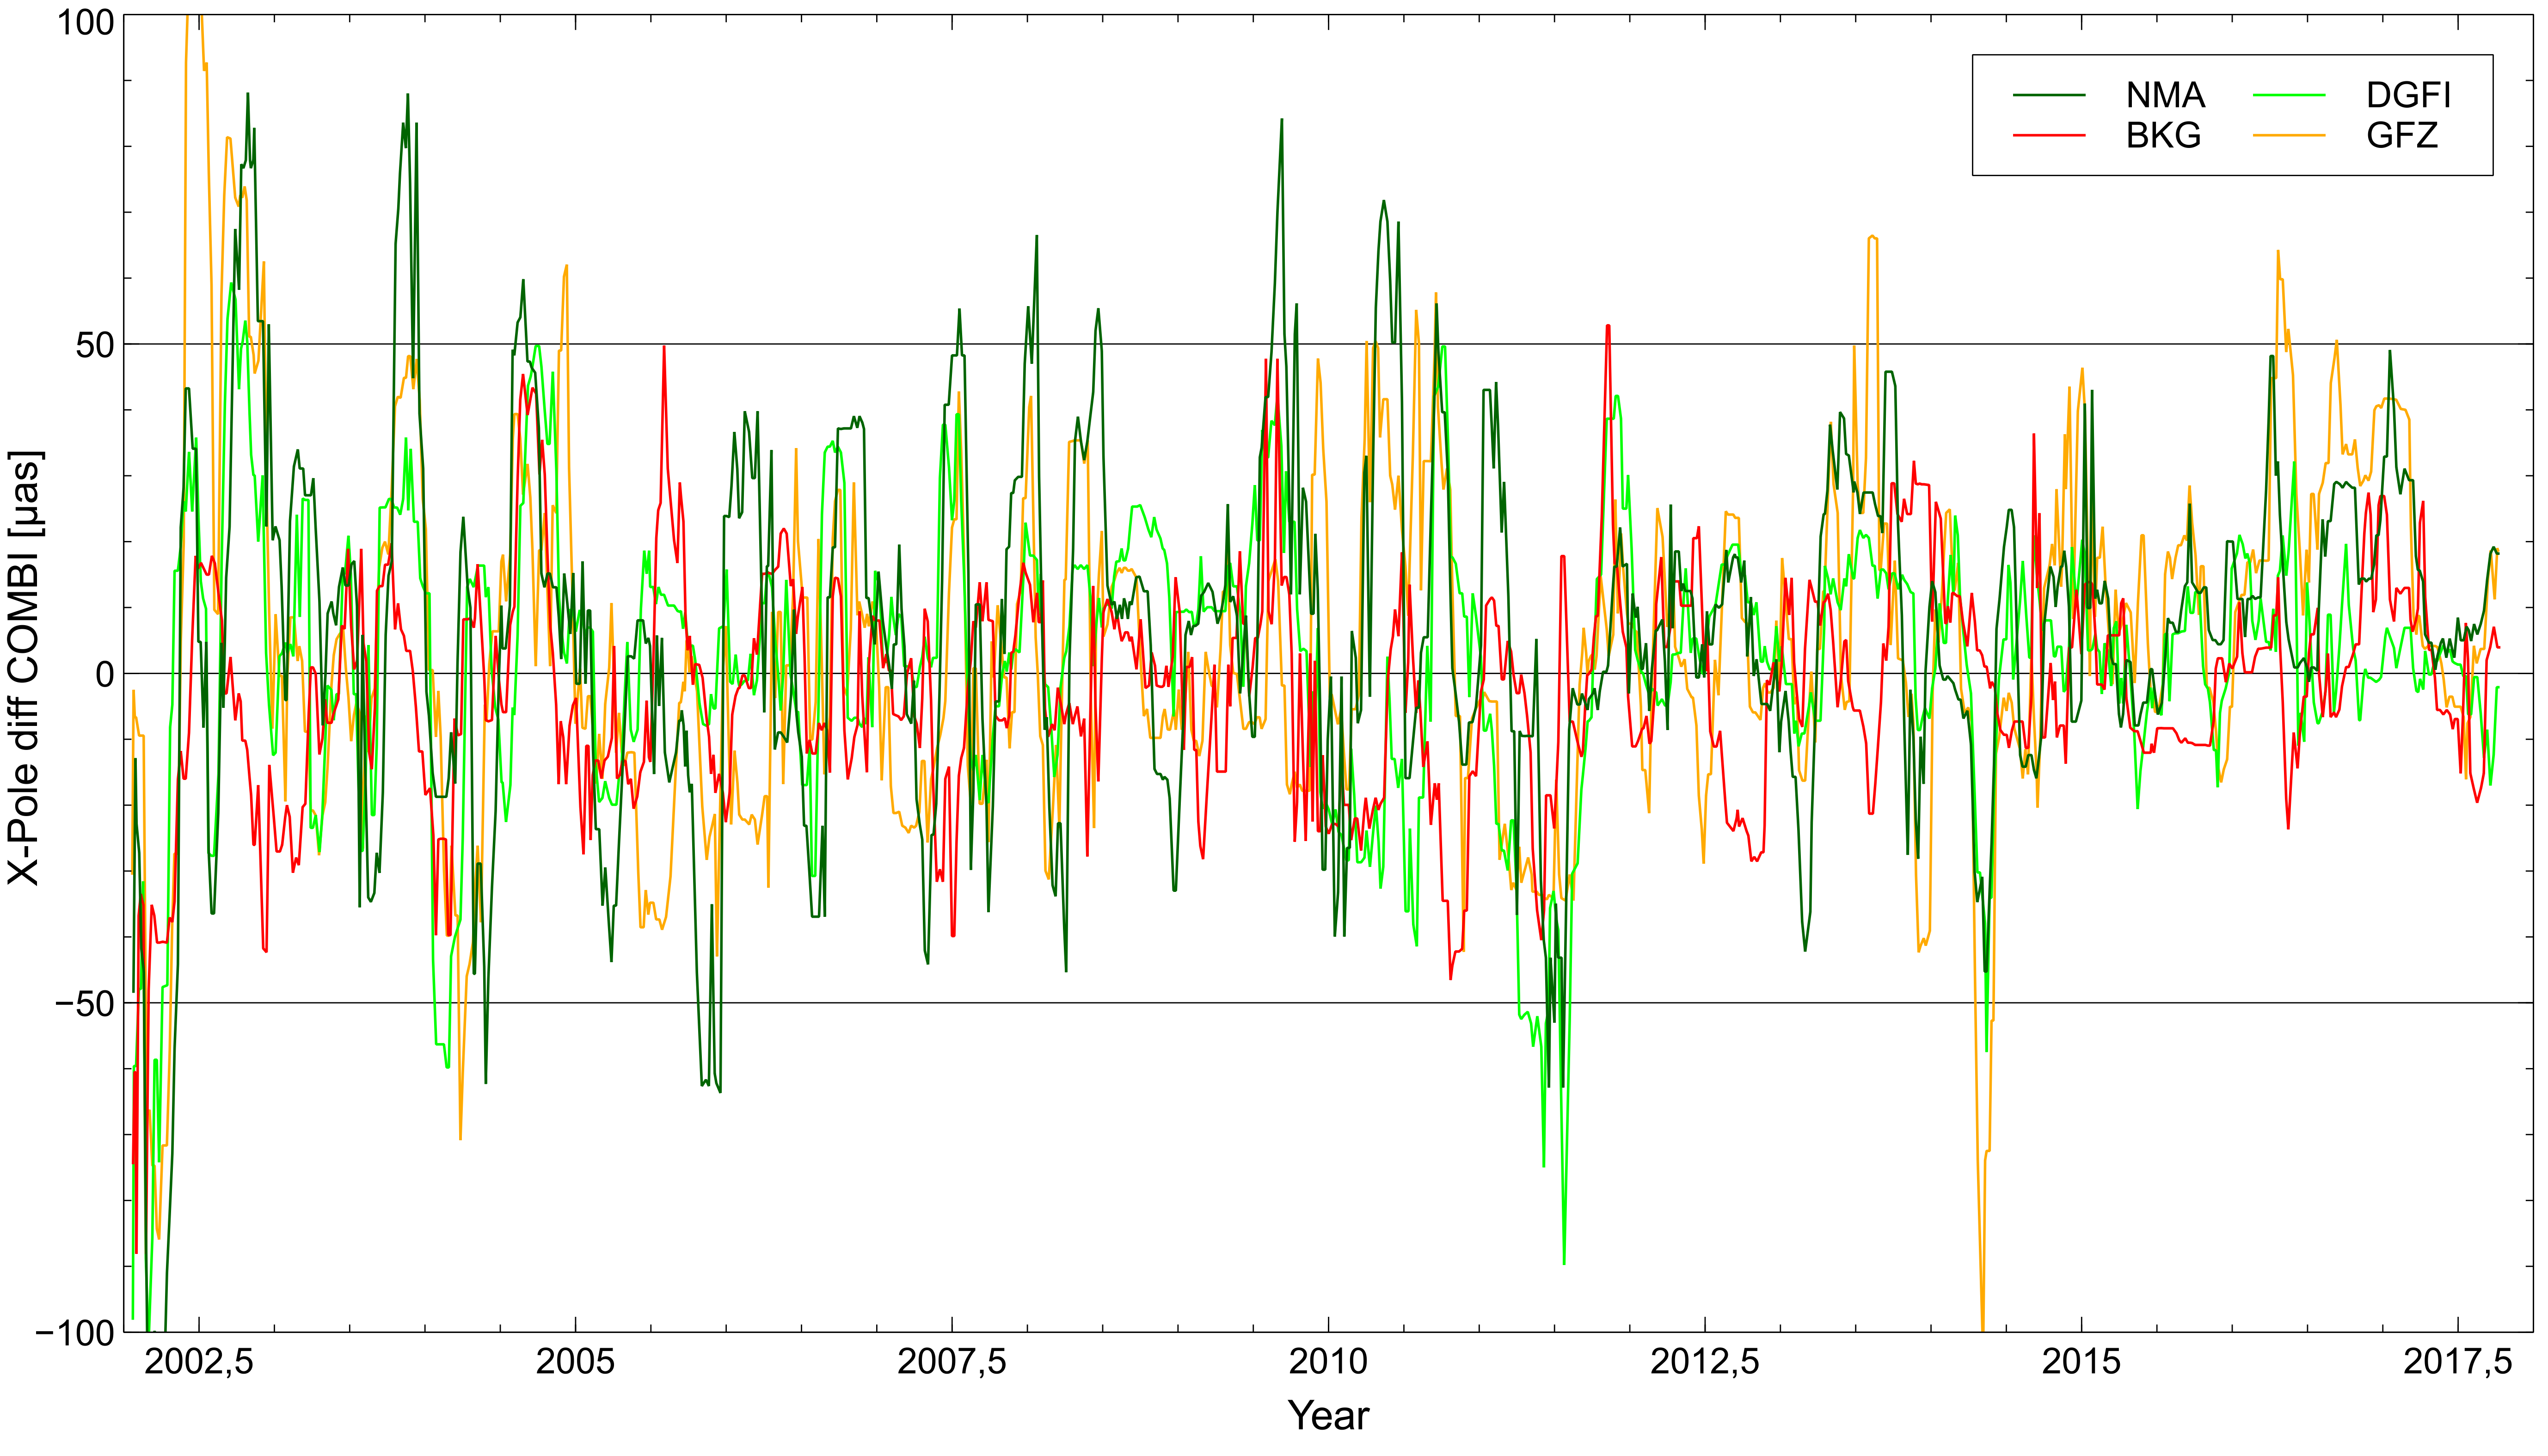
\includegraphics[width=\linewidth]{figure/iter6_x-pole_nma_diff_combi}\hspace*{\fill}
\end{centering}
\end{frame}

\begin{frame}{6. leveranse - y-pole}
\begin{centering}
    \hfill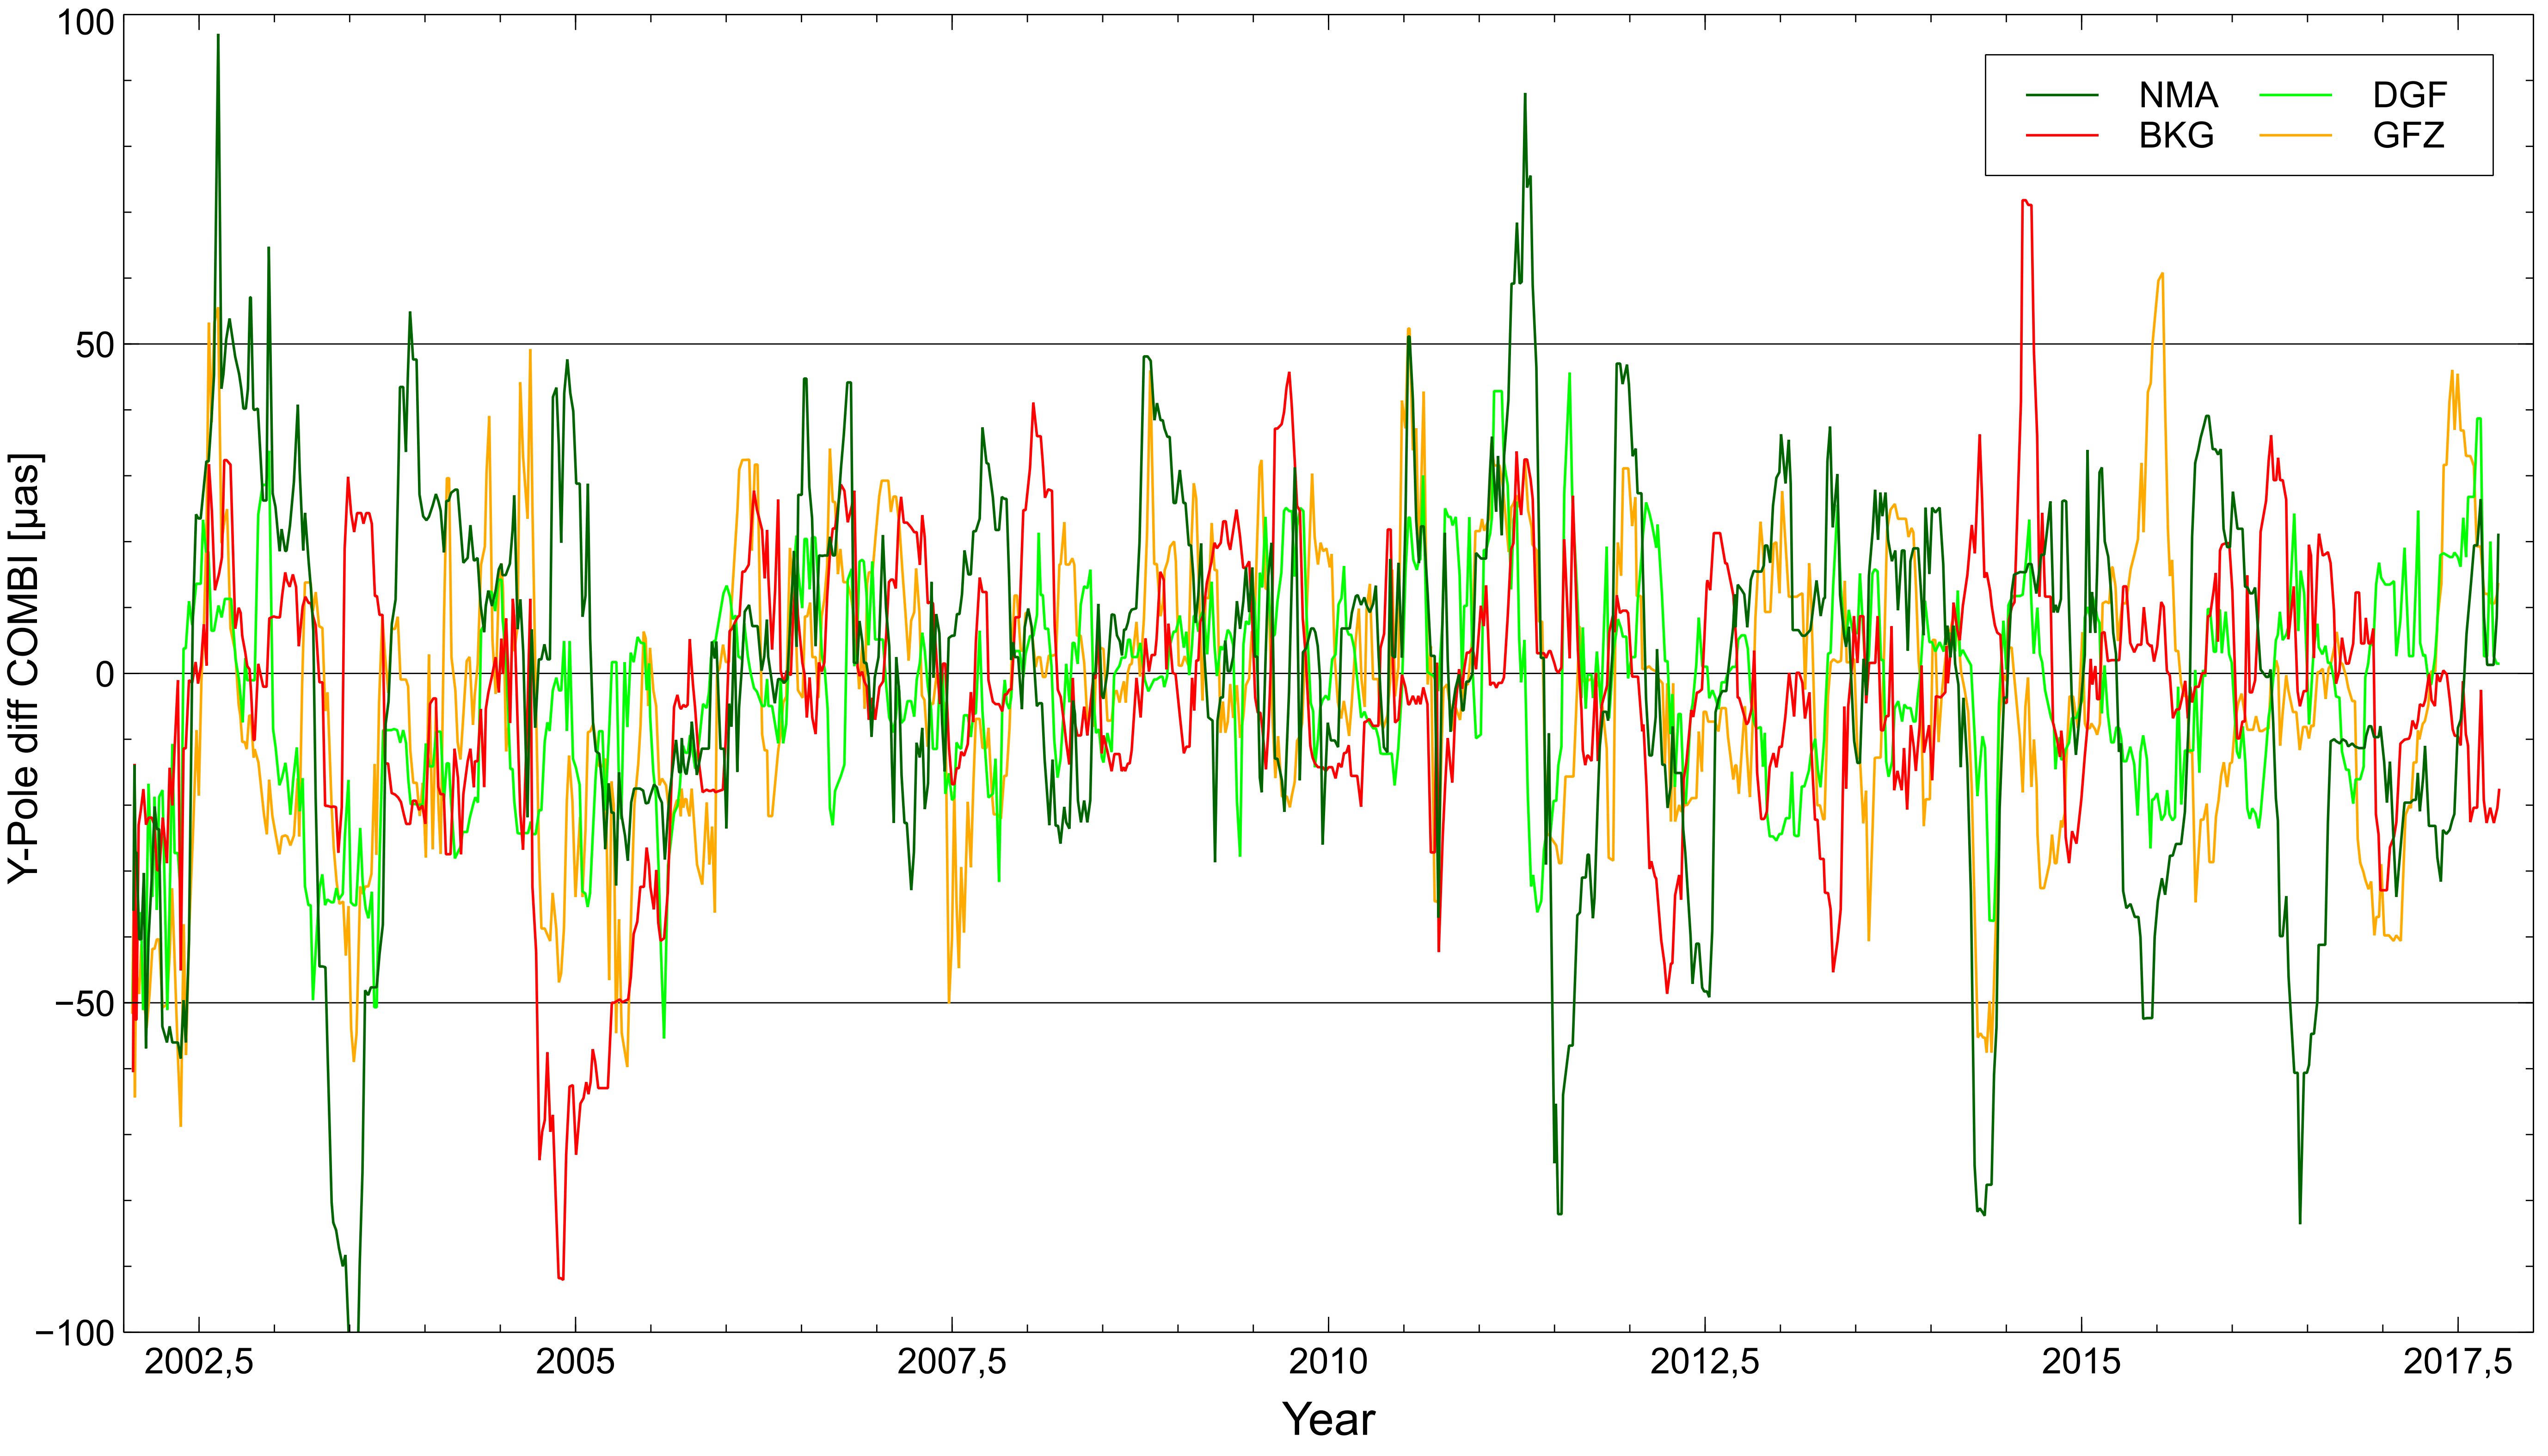
\includegraphics[width=\linewidth]{figure/iter6_y-pole_nma_diff_combi}\hspace*{\fill}
\end{centering}
\end{frame}

\begin{frame}{6. leveranse - x-pole rate}
\begin{centering}
    \hfill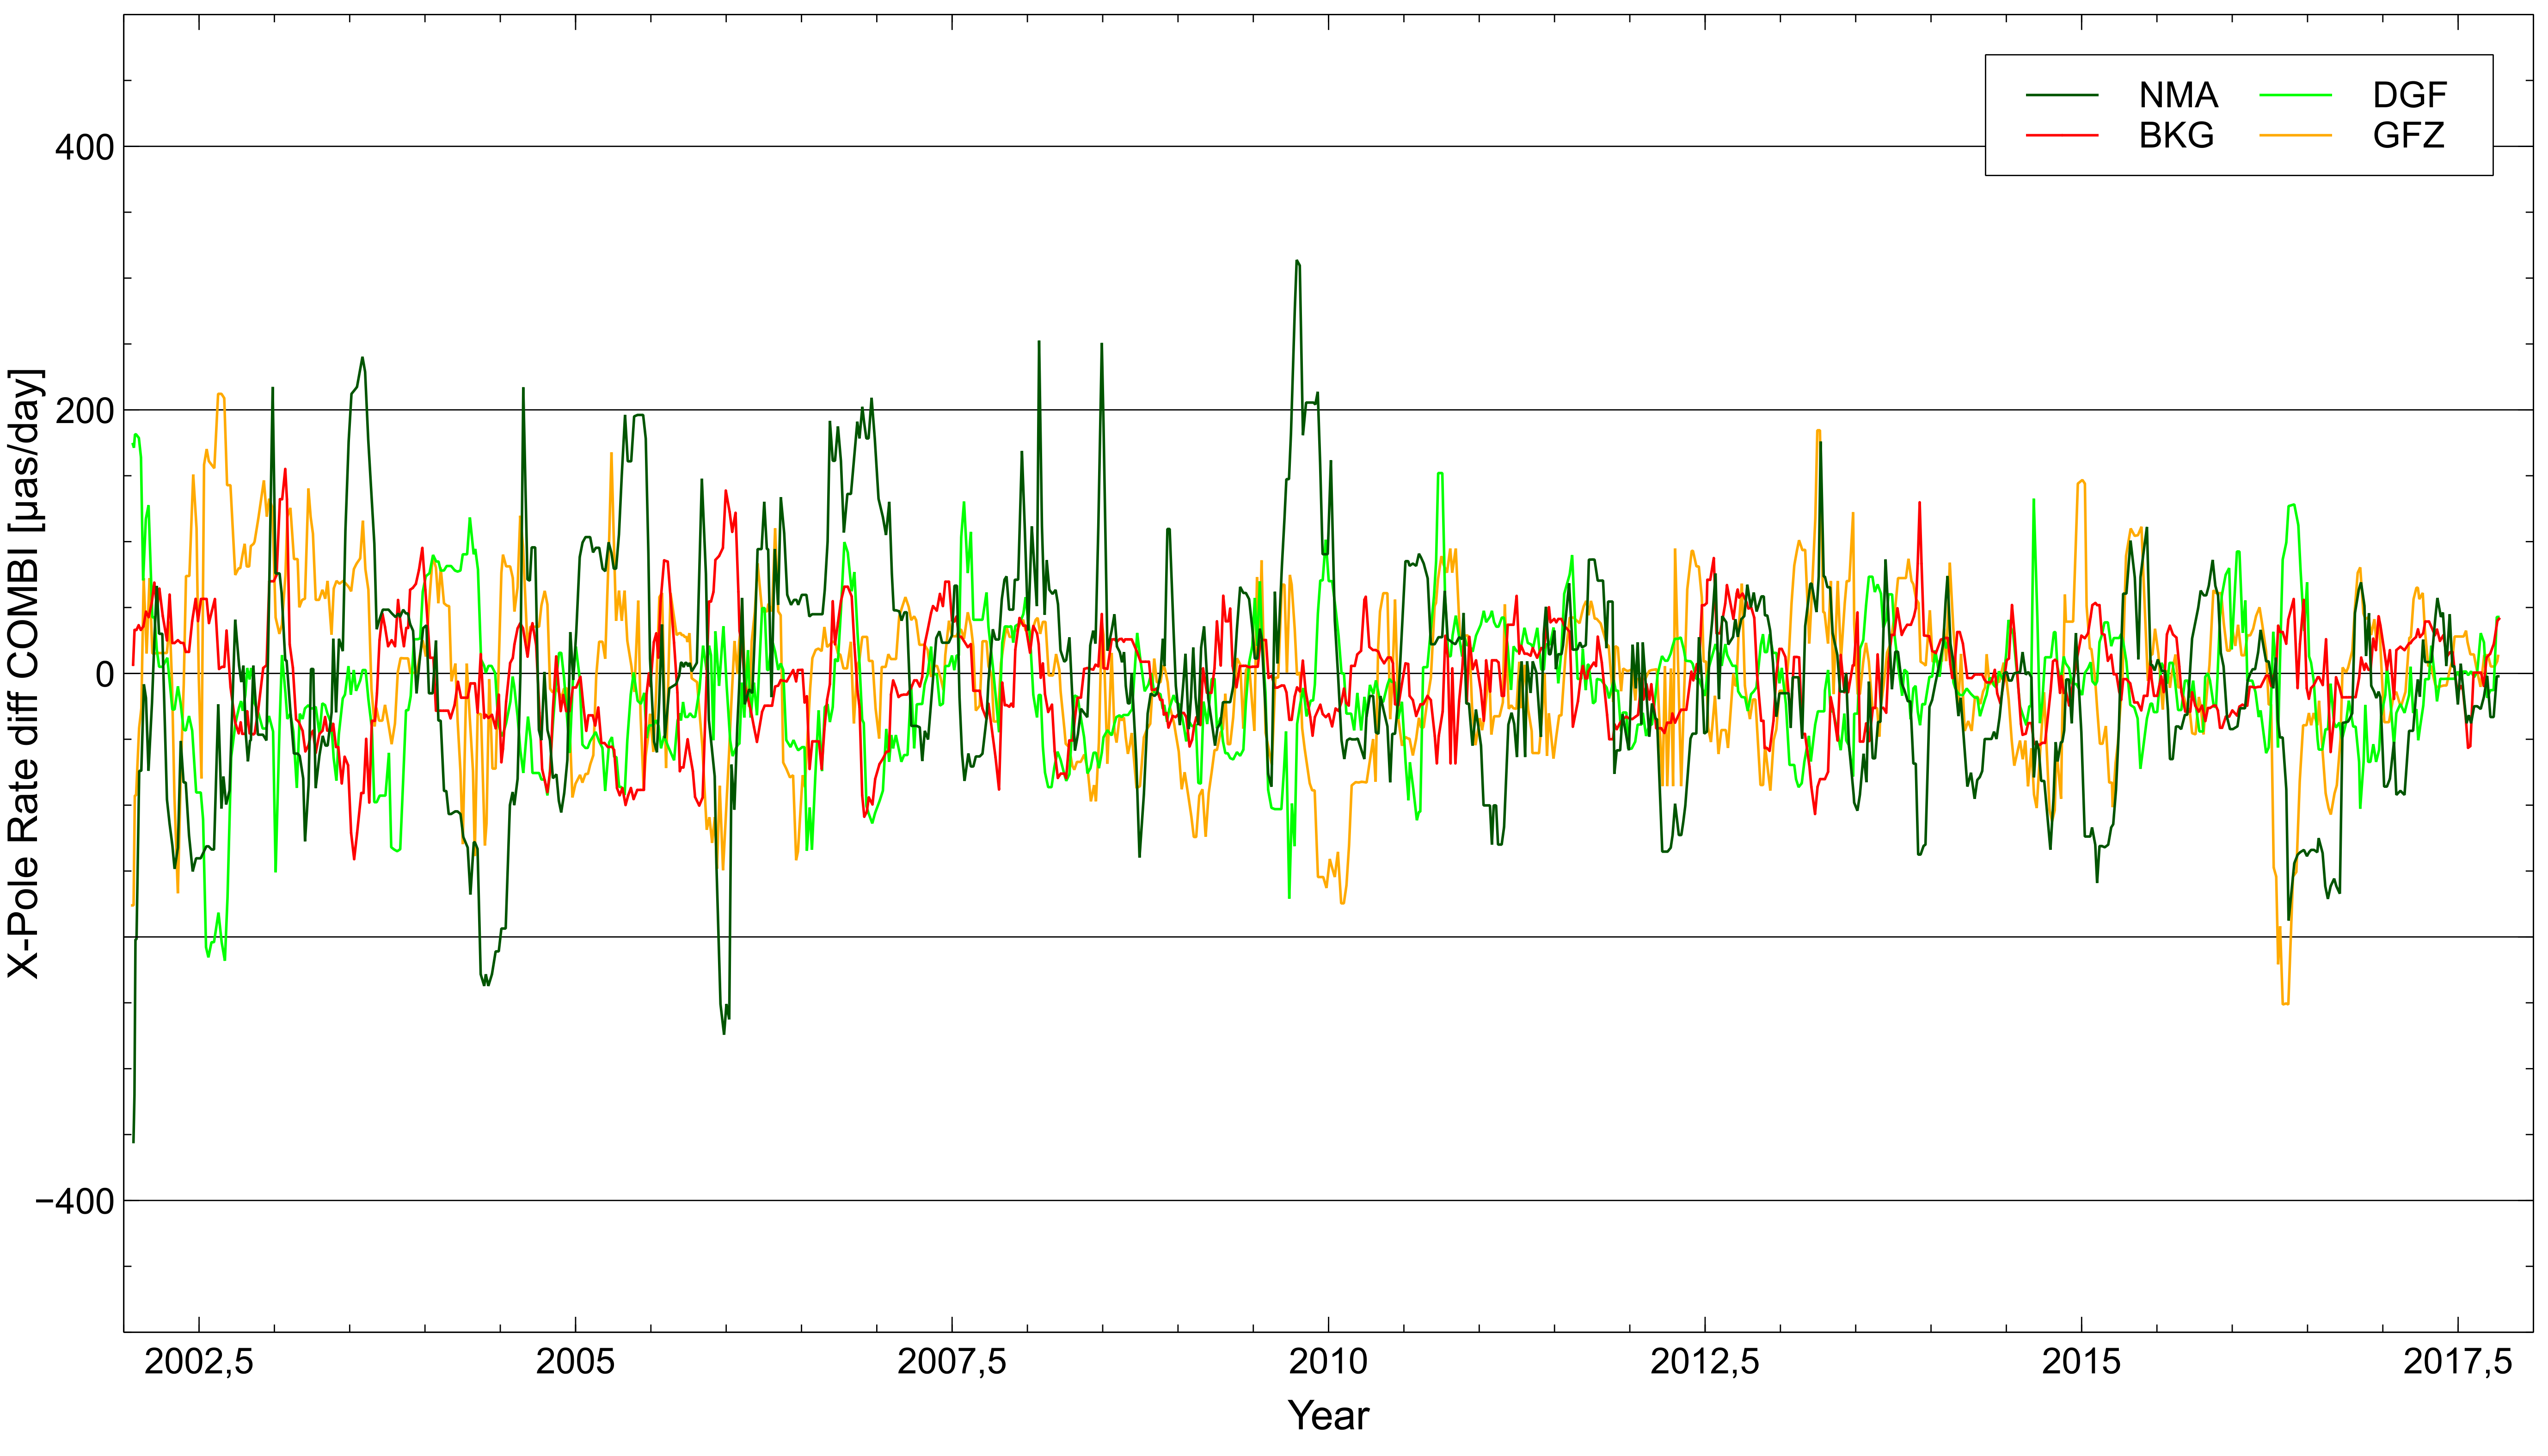
\includegraphics[width=\linewidth]{figure/iter6_x-pole-rate_nma_diff_combi}\hspace*{\fill}
\end{centering}
\end{frame}

\begin{frame}{6. leveranse - y-pole rate}
\begin{centering}
    \hfill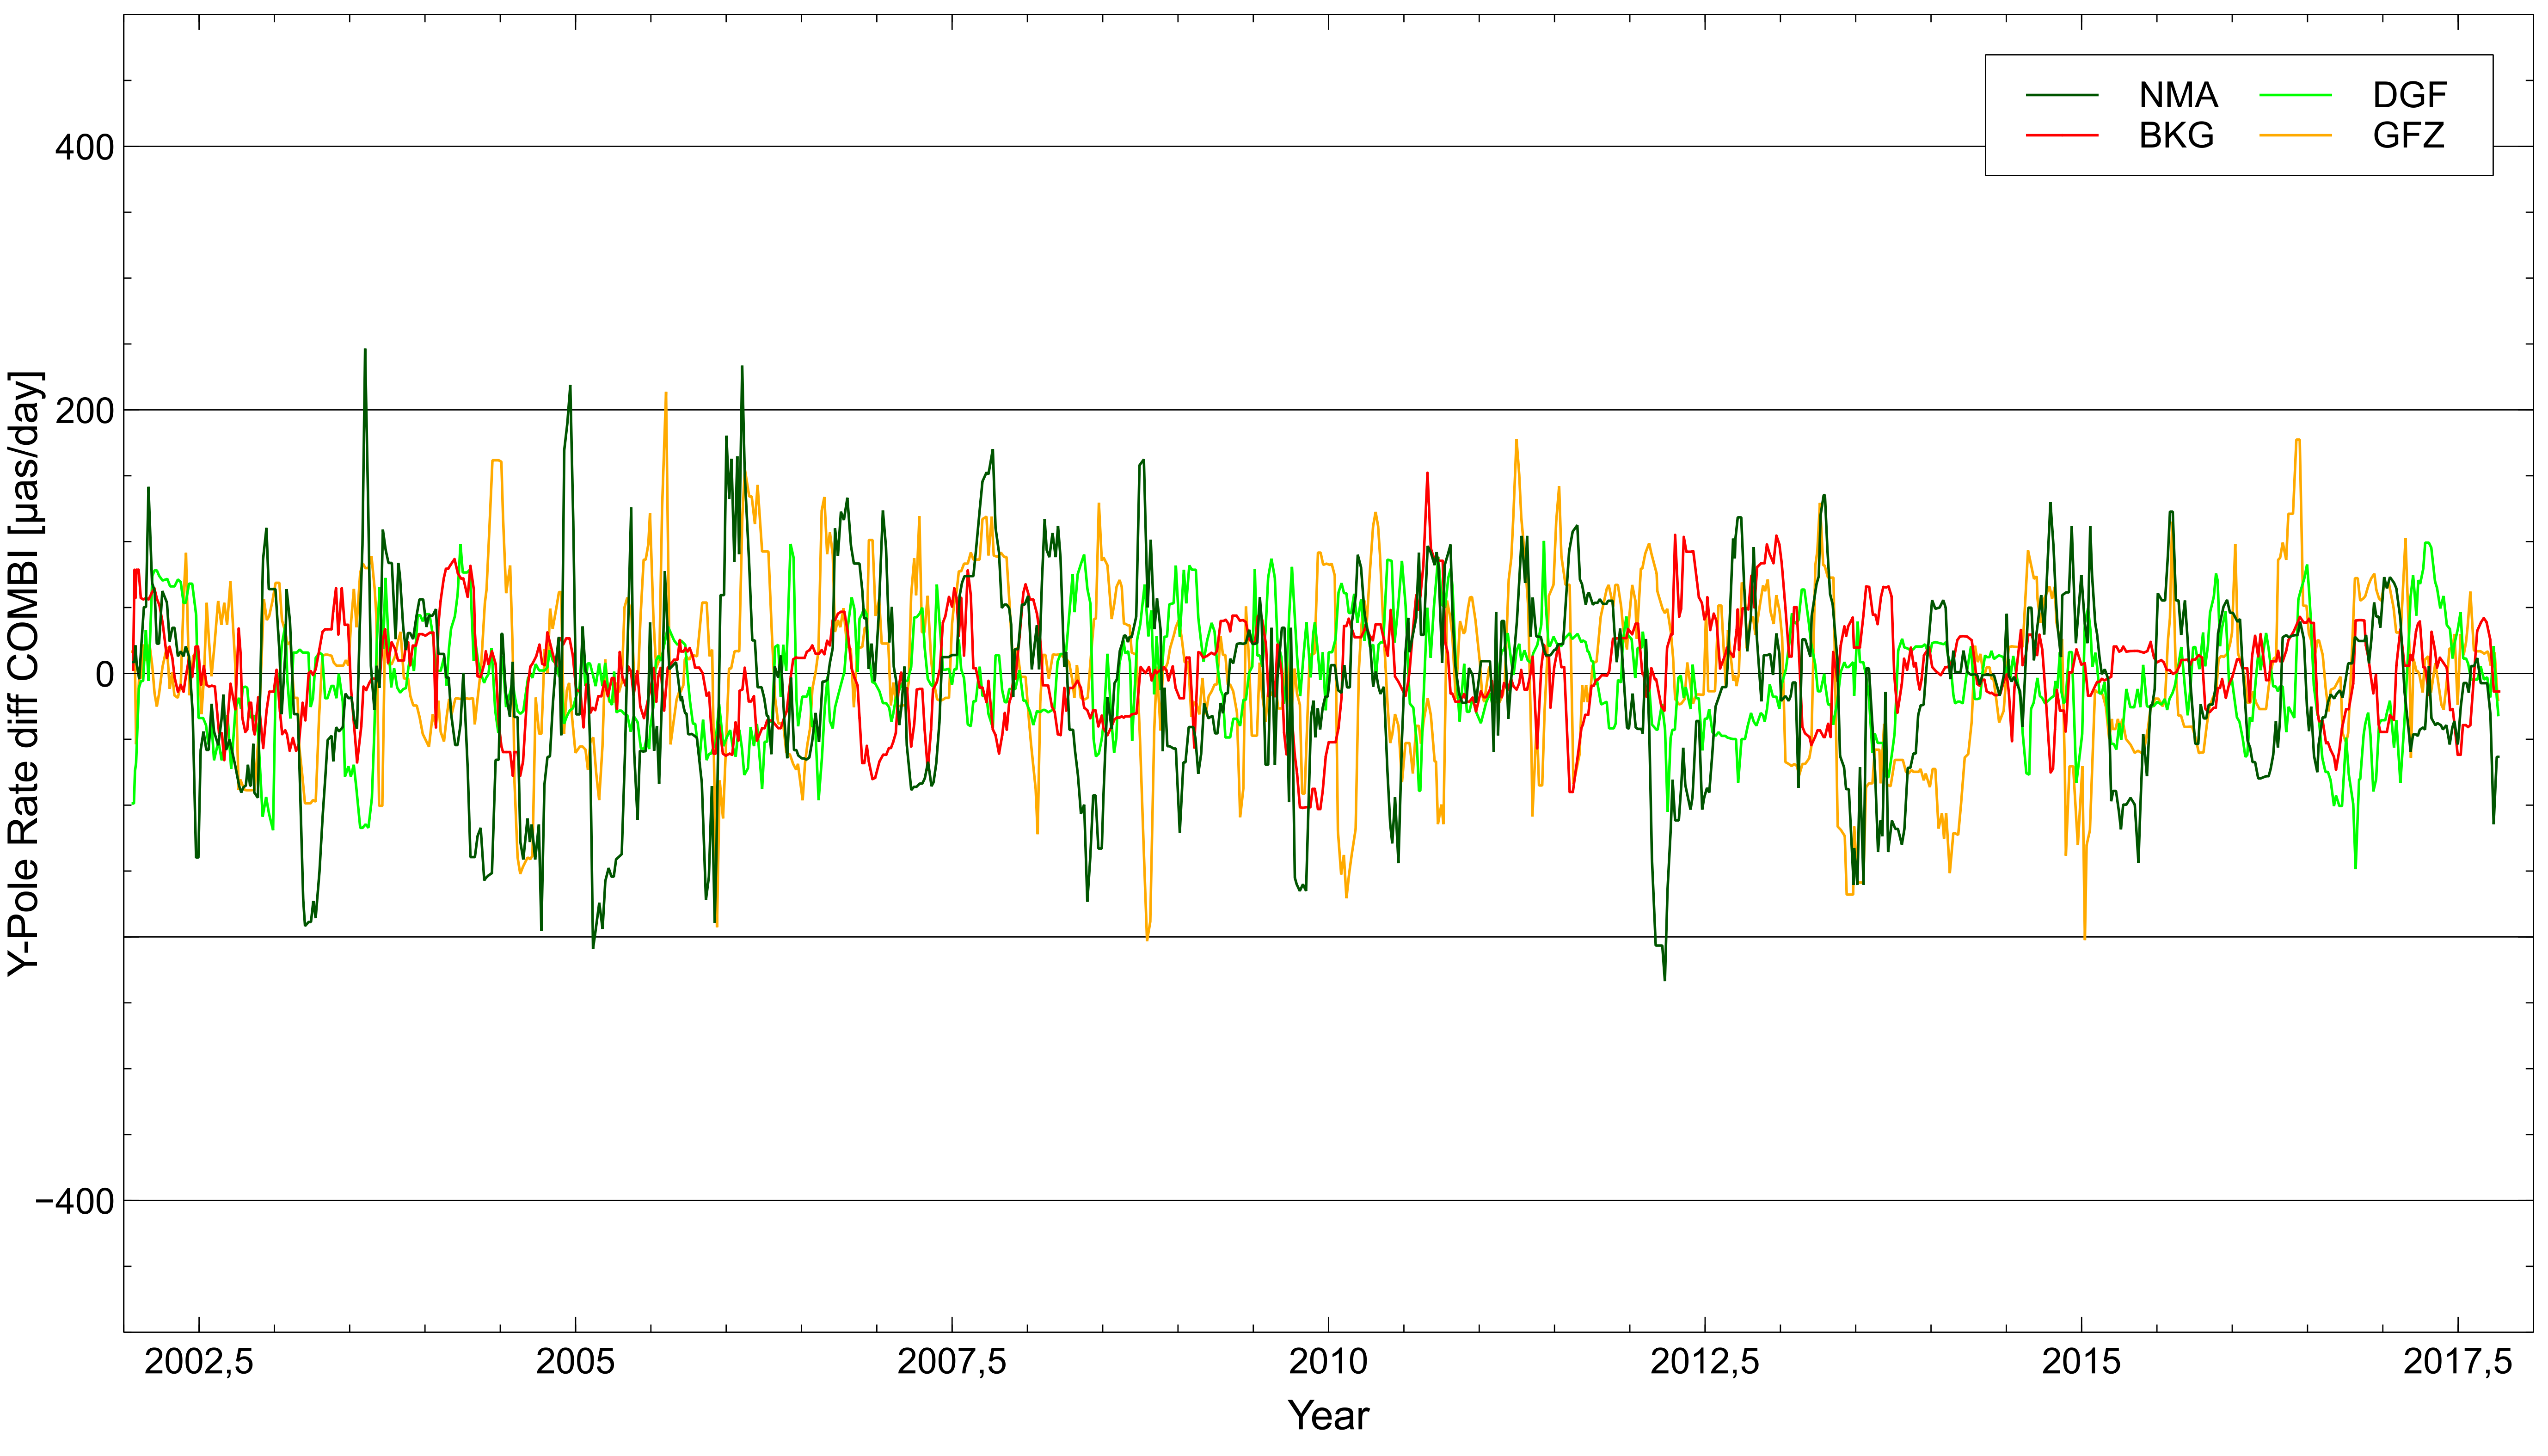
\includegraphics[width=\linewidth]{figure/iter6_y-pole-rate_nma_diff_combi}\hspace*{\fill}
\end{centering}
\end{frame}


\begin{frame}{Internasjonalt samarbeid}
\begin{itemize}
  \item Kartverket samarbeider med IGN i Spania
  \item IGN tilbyr hardware og support til Ny-Ålesund
  \item Kartverket tilbyr analyseprogram med opplæring 
\end{itemize}
\end{frame}

\begin{frame}{IGN workshop}
\begin{centering}
    \hfill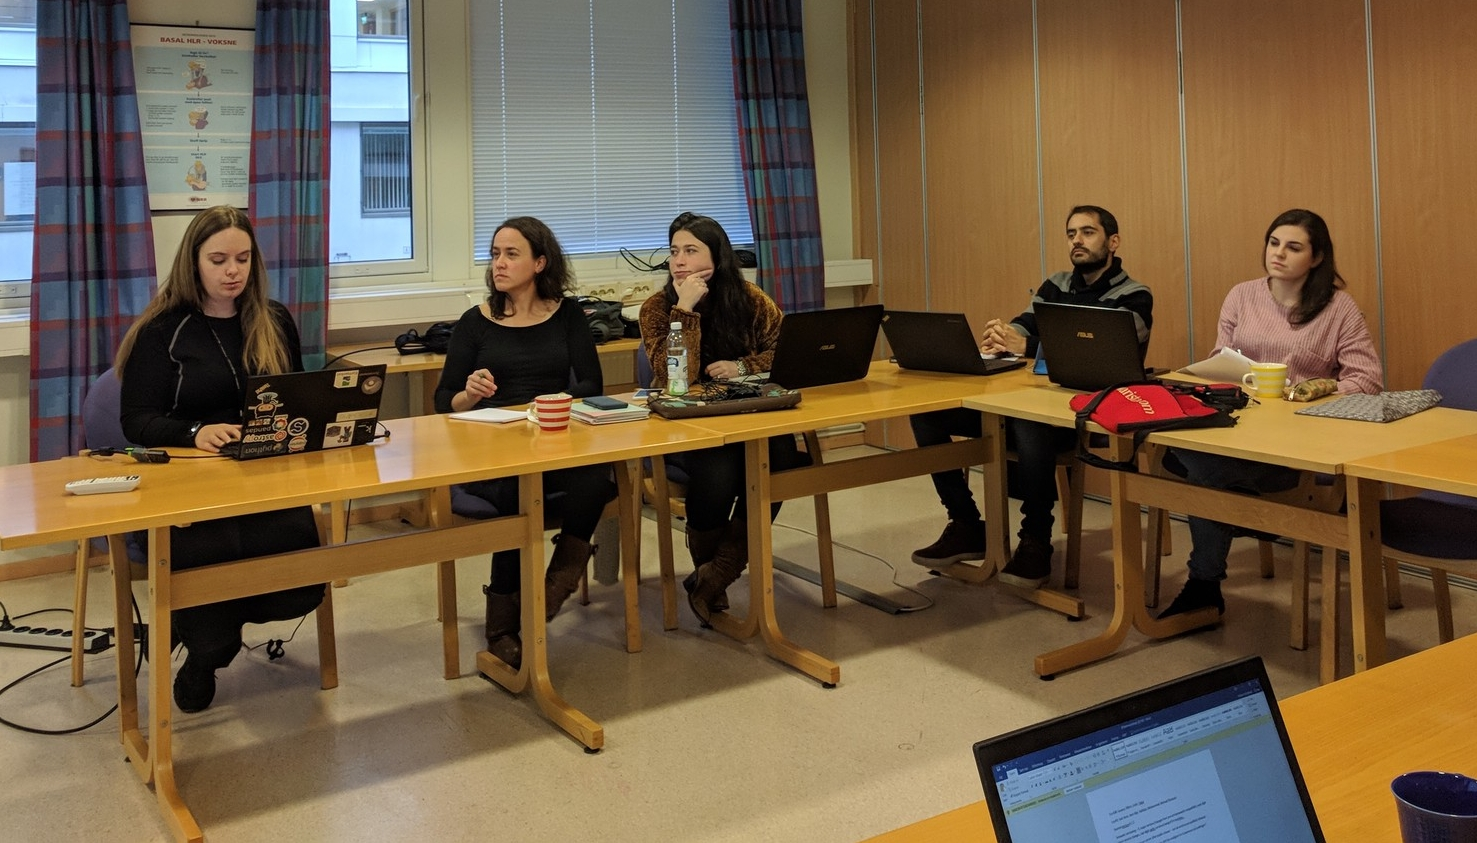
\includegraphics[width=\linewidth]{figure/workshop.jpg}\hspace*{\fill}
\end{centering}
\end{frame}


\begin{frame}{Oppsummert}
  \begin{centering}
    Hovedfokus fremover:
  \end{centering}

  \begin{itemize}
    \item Fullføre og slippe version 1.0 av \textbf{Where}
    \item Få i gang operasjonell analyse på kontrollsenteret
    \item Oppfylle vår del av avtalen med IGN
  \end{itemize}
\end{frame}


\end{document}
